% A LaTeX template for MSc Thesis submissions to 
% Politecnico di Milano (PoliMi) - School of Industrial and Information Engineering
%
% S. Bonetti, A. Gruttadauria, G. Mescolini, A. Zingaro
% e-mail: template-tesi-ingind@polimi.it
%
% Last Revision: October 2021
%
% Copyright 2021 Politecnico di Milano, Italy. NC-BY

\documentclass{Configuration_Files/PoliMi3i_thesis}

%------------------------------------------------------------------------------
%	REQUIRED PACKAGES AND  CONFIGURATIONS
%------------------------------------------------------------------------------

% CONFIGURATIONS
\usepackage{parskip} % For paragraph layout
\usepackage{setspace} % For using single or double spacing
\usepackage{emptypage} % To insert empty pages
\usepackage{multicol} % To write in multiple columns (executive summary)
\setlength\columnsep{15pt} % Column separation in executive summary
\setlength\parindent{0pt} % Indentation
\raggedbottom  

% PACKAGES FOR TITLES
\usepackage{titlesec}
% \titlespacing{\section}{left spacing}{before spacing}{after spacing}
\titlespacing{\section}{0pt}{3.3ex}{2ex}
\titlespacing{\subsection}{0pt}{3.3ex}{1.65ex}
\titlespacing{\subsubsection}{0pt}{3.3ex}{1ex}
\usepackage{color}

% PACKAGES FOR LANGUAGE AND FONT
\usepackage[english]{babel} % The document is in English  
\usepackage[utf8]{inputenc} % UTF8 encoding
\usepackage[T1]{fontenc} % Font encoding
\usepackage[11pt]{moresize} % Big fonts

% PACKAGES FOR IMAGES
\usepackage{graphicx}
\usepackage{transparent} % Enables transparent images
\usepackage{eso-pic} % For the background picture on the title page
\usepackage{subfig} % Numbered and caption subfigures using \subfloat.
\usepackage{tikz} % A package for high-quality hand-made figures.
\usetikzlibrary{}
\graphicspath{{./Images/}} % Directory of the images
\usepackage{caption} % Coloured captions
\usepackage{xcolor} % Coloured captions
\usepackage{amsthm,thmtools,xcolor} % Coloured "Theorem"
\usepackage{float}

% STANDARD MATH PACKAGES
\usepackage{amsmath}
\usepackage{amsthm}
\usepackage{amssymb}
\usepackage{amsfonts}
\usepackage{bm}
\usepackage[overload]{empheq} % For braced-style systems of equations.
\usepackage{fix-cm} % To override original LaTeX restrictions on sizes

% PACKAGES FOR TABLES
\usepackage{tabularx}
\usepackage{longtable} % Tables that can span several pages
\usepackage{colortbl}

% PACKAGES FOR ALGORITHMS (PSEUDO-CODE)
\usepackage{algorithm}
\usepackage{algorithmic}

% PACKAGES FOR REFERENCES & BIBLIOGRAPHY
\usepackage[colorlinks=true,linkcolor=black,anchorcolor=black,citecolor=black,filecolor=black,menucolor=black,runcolor=black,urlcolor=black]{hyperref} % Adds clickable links at references
\usepackage{cleveref}
\usepackage[square, numbers, sort&compress]{natbib} % Square brackets, citing references with numbers, citations sorted by appearance in the text and compressed
\bibliographystyle{abbrvnat} % You may use a different style adapted to your field

% OTHER PACKAGES
\usepackage{pdfpages} % To include a pdf file
\usepackage{afterpage}
\usepackage{lipsum} % DUMMY PACKAGE
\usepackage{fancyhdr} % For the headers
\fancyhf{}

% Input of configuration file. Do not change config.tex file unless you really know what you are doing. 
% Define blue color typical of polimi
\definecolor{bluepoli}{cmyk}{0.4,0.1,0,0.4}

% Custom theorem environments
\declaretheoremstyle[
  headfont=\color{bluepoli}\normalfont\bfseries,
  bodyfont=\color{black}\normalfont\itshape,
]{colored}

% Set-up caption colors
\captionsetup[figure]{labelfont={color=bluepoli}} % Set colour of the captions
\captionsetup[table]{labelfont={color=bluepoli}} % Set colour of the captions
\captionsetup[algorithm]{labelfont={color=bluepoli}} % Set colour of the captions

\theoremstyle{colored}
\newtheorem{theorem}{Theorem}[chapter]
\newtheorem{proposition}{Proposition}[chapter]

% Enhances the features of the standard "table" and "tabular" environments.
\newcommand\T{\rule{0pt}{2.6ex}}
\newcommand\B{\rule[-1.2ex]{0pt}{0pt}}

% Pseudo-code algorithm descriptions.
\newcounter{algsubstate}
\renewcommand{\thealgsubstate}{\alph{algsubstate}}
\newenvironment{algsubstates}
  {\setcounter{algsubstate}{0}%
   \renewcommand{\STATE}{%
     \stepcounter{algsubstate}%
     \Statex {\small\thealgsubstate:}\space}}
  {}

% New font size
\newcommand\numfontsize{\@setfontsize\Huge{200}{60}}

% Title format: chapter
\titleformat{\chapter}[hang]{
\fontsize{50}{20}\selectfont\bfseries\filright}{\textcolor{bluepoli} \thechapter\hsp\hspace{2mm}\textcolor{bluepoli}{|   }\hsp}{0pt}{\huge\bfseries \textcolor{bluepoli}
}

% Title format: section
\titleformat{\section}
{\color{bluepoli}\normalfont\Large\bfseries}
{\color{bluepoli}\thesection.}{1em}{}

% Title format: subsection
\titleformat{\subsection}
{\color{bluepoli}\normalfont\large\bfseries}
{\color{bluepoli}\thesubsection.}{1em}{}

% Title format: subsubsection
\titleformat{\subsubsection}
{\color{bluepoli}\normalfont\large\bfseries}
{\color{bluepoli}\thesubsubsection.}{1em}{}

% Shortening for setting no horizontal-spacing
\newcommand{\hsp}{\hspace{0pt}}

\makeatletter
% Renewcommand: cleardoublepage including the background pic
\renewcommand*\cleardoublepage{%
  \clearpage\if@twoside\ifodd\c@page\else
  \null
  \AddToShipoutPicture*{\BackgroundPic}
  \thispagestyle{empty}%
  \newpage
  \if@twocolumn\hbox{}\newpage\fi\fi\fi}
\makeatother

%For correctly numbering algorithms
\numberwithin{algorithm}{chapter}

%----------------------------------------------------------------------------
%	NEW COMMANDS DEFINED
%----------------------------------------------------------------------------

% EXAMPLES OF NEW COMMANDS
\newcommand{\bea}{\begin{eqnarray}} % Shortcut for equation arrays
\newcommand{\eea}{\end{eqnarray}}
\newcommand{\e}[1]{\times 10^{#1}}  % Powers of 10 notation

%----------------------------------------------------------------------------
%	ADD YOUR PACKAGES (be careful of package interaction)
%----------------------------------------------------------------------------
\usepackage{listings}
%----------------------------------------------------------------------------
%	ADD YOUR DEFINITIONS AND COMMANDS (be careful of existing commands)
%----------------------------------------------------------------------------
\definecolor{codegreen}{rgb}{0,0.6,0}
\definecolor{codegray}{rgb}{0.5,0.5,0.5}
\definecolor{codepurple}{rgb}{0.58,0,0.82}
\definecolor{backcolour}{rgb}{0.95,0.95,0.92}

\lstdefinestyle{mystyle}{
    backgroundcolor=\color{backcolour},   
    commentstyle=\color{codegreen},
    keywordstyle=\color{magenta},
    numberstyle=\tiny\color{codegray},
    stringstyle=\color{codepurple},
    basicstyle=\ttfamily\footnotesize,
    breakatwhitespace=false,         
    breaklines=true,                 
    captionpos=b,                    
    keepspaces=true,                 
    numbers=left,                    
    numbersep=5pt,                  
    showspaces=false,                
    showstringspaces=false,
    showtabs=false,                  
    tabsize=2
}
\lstset{style=mystyle}

\let\phi\varphi
\let\epsilon\varepsilon
%----------------------------------------------------------------------------
%	BEGIN OF YOUR DOCUMENT
%----------------------------------------------------------------------------

\begin{document}

\fancypagestyle{plain}{%
\fancyhf{} % Clear all header and footer fields
\fancyhead[RO,RE]{\thepage} %RO=right odd, RE=right even
\renewcommand{\headrulewidth}{0pt}
\renewcommand{\footrulewidth}{0pt}}

%----------------------------------------------------------------------------
%	TITLE PAGE
%----------------------------------------------------------------------------

%\pagestyle{empty} % No page numbers
%\frontmatter % Use roman page numbering style (i, ii, iii, iv...) for the preamble pages

\puttitle{
	title=Transient simulation of charge accumulation in HVDC cables
during switching, % Title of the thesis
	name=Alessandro Lombardi, % Author Name and Surname
	course=\\Project Report, % Study Programme (in Italian)
	ID  = 946444,  % Student ID number (numero di matricola)
	advisor= Prof. Carlo De Falco, % Supervisor name
	academicyear={2021-22},  % Academic Year
} % These info will be put into your Title page 

%----------------------------------------------------------------------------
%	PREAMBLE PAGES: ABSTRACT (inglese e italiano), EXECUTIVE SUMMARY
%----------------------------------------------------------------------------
%\startpreamble
%\setcounter{page}{1} % Set page counter to 1


%----------------------------------------------------------------------------
%	LIST OF CONTENTS/FIGURES/TABLES/SYMBOLS
%----------------------------------------------------------------------------

% TABLE OF CONTENTS
%\thispagestyle{empty}
\tableofcontents % Table of contents 
%\thispagestyle{empty}


%-------------------------------------------------------------------------
%	THESIS MAIN TEXT
%-------------------------------------------------------------------------
% In the main text of your thesis you can write the chapters in two different ways:
%
%(1) As presented in this template you can write:
%    \chapter{Title of the chapter}
%    *body of the chapter*
%
%(2) You can write your chapter in a separated .tex file and then include it in the main file with the following command:
%    \chapter{Title of the chapter}
%    \input{chapter_file.tex}
%
% Especially for long thesis, we recommend you the second option.

\addtocontents{toc}{\vspace{2em}} % Add a gap in the Contents, for aesthetics
%\mainmatter % Begin numeric (1,2,3...) page numbering

% --------------------------------------------------------------------------
% NUMBERED CHAPTERS % Regular chapters following
% --------------------------------------------------------------------------
\chapter*{Introduction}
High Voltage Direct Current (HVDC) is an electric power transmission system commonly used to transmit power over long distances and for undersea cables, making it ideal for offshore windfarms. Other uses include connecting unsynchronized AC grids to each other, such as the ones of neighbouring countries. It requires a converter-transformer at each end in order to connect it to the local AC grid, however, due to the absence of skin effect transmission, losses are 50\% less than AC lines at the same voltage. Moreover HVDC requires less conductor per unit distance than an AC line since there is no need to support three phases. 
\\The standard structure of the cable for HDVC consist of a coaxial cable surrounded by an insulation layer made by high-pressure oil or of mass impregnated paper with high-viscosity insulating compound.\cite{reportEU} In both these cases, any damage to the cable which causes leakage of the fluid will need expensive repairs before being able to be used again. 
\\In more recent years, polymeric materials have been used as insulators in HVDC applications. These so-called extruded cables have the advantage of being smaller and lighter, moreover they are not subjects to leakage and don't require additional equipment to maintain the fluid pressure. A disadvantage of these insulating materials is that the insulation of such cables exhibit complex non-linear conduction current (charge transport in dielectric) when used under high DC stress \cite{cable}. The conduction current is also considered responsible for the space charge accumulation, which is claimed to be the main factor accelerating degradation of polymeric insulation in HVDC cables with respect to HVAC \cite{cable2}. This is the reason why understanding the dominant chemical and physical processes in the insulation, achieved through experiments, development of theoretical models and numerical simulations, can help to build reliable systems.
\\The goal of this project is to study the electric charge distribution in HVDC insulation materials in non-stationary conditions. We first develop a relatively simple numerical model for evaluating the behavior of the electric field and the space charge inside the insulator. Then we implement it using the bim++ library.

This report is structured as follows. In Chapter 1 the mathematical model is derived and discussed. Chapter 2 focuses on the coding aspect of the project. Finally in Chapter 3 we present the numerical results.


\chapter{Mathematical Model}
\section{Derivation of the equations}
The following mathematical model will be derived under the quasi-electrostatic approximation:
\begin{equation}
    \label{eq: qea}
    \nabla \times \bm{E}=0
\end{equation}
where $\bm{E}$ is the electric field. This allows us to introduce a scalar potential $\phi$ such that
\begin{equation}
    \label{eq: campo}
    \bm{E}=-\nabla  \phi
\end{equation}
Under the same assumption, let's now consider Maxwell's equations:
% \begin{equation}
%     \label{eq: Gauss}
%     \nabla \cdot \bm{D}=\rho
% \end{equation}

\begin{subequations}
    \label{eq:maxwell}
    \begin{align}
    \nabla\cdot \bm{D} & = \rho, \label{eq: Gauss} \\
    \nabla \times \bm{H} - \frac{\partial \bm{D}}{\partial t} &= \bm{J}. \label{eq: Max4}
    \end{align}
\end{subequations}

Equation \ref{eq: Gauss}, also known as Gauss' law, relates the dielectric displacement vector $\bm{D}$ to the net density of charge per unit volume $\rho$. 
\\Inside a dielectric material the displacement vector is given by
\begin{equation}
    \label{eq: dielectric}
    \bm{D}=\epsilon_0 \bm{E} +\bm{P}
\end{equation}
where $\epsilon_0$ is the vacuum permittivity and  $\bm{P}$ is the polarization vector which we can assume to be due to a number of different processes, each behaving according to the Debye relaxation model \cite{Debye}
\begin{equation}
    \label{eq: Debye}
    \bm{P}=\bm{P}_\infty + \sum_k \bm{P}_k
\end{equation}
where
\begin{equation}
    \label{eq: Debye 2}
    \bm{P}_\infty = \epsilon_0\chi_\infty\bm{E}
\end{equation}
and each of the contributions $\bm{P}_k$ obeys a relaxation–type ordinary differential equation of the form
\begin{equation}
    \label{eq: Debye 3}
    \tau_k\frac{\partial}{\partial t}\bm{P}_k = \epsilon_0\chi_k\bm{E}-\bm{P}_k
\end{equation}
where $\tau_k$ is the corresponding time constant and the parameter $\chi_k$ represent the electric susceptibility for a given frequency component $k$.
\\It has been shown that this model for the polarization can correctly represent currents in impregnated-paper  insulation during  transients regimes \cite{Cambieri}. However, it becomes much less accurate when applied to polymeric materials such as polypropylene. The different behaviour observed in polymeric material can be ascribed to the the presence of charge carrier traps in such materials. \\To account for this phenomenon, let model the charge density $\rho$ as 
\begin{equation}
    \label{eq: rho}
    \rho=q(p-n+b)
\end{equation}
where $p$ are the (positively charged) mobile charges, b are the (positively charged) trapped charges and n the (negatively) charged trap states. We assume the trap states to be fixed 
\begin{equation}
    \label{eq: n}
    \frac{\partial n}{\partial t}=0
\end{equation}
while the model for charge trapping will be discussed later
\begin{equation}
    \label{eq: b}
    \frac{\partial b}{\partial t}=\Dot{b}(\bm{J},b)
\end{equation}
\\Let's now consider equation \ref{eq: Max4}, in which $\bm{H}$ is the magnetic field strength and $\bm{J}$ is the current density. $\bm{J}$ can be expressed as a function of the electric field:
\begin{equation}
    \label{eq: J}
    \bm{J}=\sigma\bm{E}
\end{equation}
where $\sigma$ is the electrical conductivity which is a function of the electric field and the temperature:
\begin{equation}
    \label{eq: sigma}
    \sigma=(1-a)\sigma_1(|\nabla\phi|,T)+a\sigma_0(T)
\end{equation}
with
\begin{align}
    \tau_a\frac{\partial a}{\partial t} &= \Bar{a}(|\nabla\phi|)-a \label{eq: tau_a} \\
    \Bar{a}&=\begin{cases}0,& |\nabla\phi|>e_{tr}\\1,& |\nabla\phi|\le e_{tr}\end{cases} \\
    \frac{1}{\tau_a}&=\begin{cases}\frac{\kappa+1}{c}\sqrt[\leftroot{-2}\uproot{2}\kappa+1]{a(t)},& |\nabla\phi|>e_{tr}\\ \frac{1}{\Bar{\tau_a}},& |\nabla\phi|\le e_{tr}\end{cases}
\end{align}
where $\tau_a$ is the time constant and $e_{tr},\ \kappa,\ c$ and $\Bar{\tau_a}$ are constants.
\\By combining \ref{eq: campo}, \ref{eq: Gauss} and \ref{eq: dielectric} we get
\begin{equation}
    \label{eq: p1}
    \rho=\nabla\cdot\bm{D}=-\nabla\cdot(\epsilon_0\nabla\phi)+\nabla\cdot\bm{P}=-\nabla\cdot(\epsilon_0(1+\xi_\infty)\nabla\phi)+\sum_k\nabla\cdot\bm{P}_k
\end{equation}
Using \ref{eq: rho} and $\epsilon_\infty=1+\chi_\infty$, \ref{eq: p1} becomes 
\begin{equation}
    \label{eq: p2}
    -\nabla\cdot(\epsilon_0\epsilon_\infty\nabla\phi)=q(p-n-b)-\sum_k\nabla\cdot\bm{P}_k
\end{equation}
If we now take the divergence of \ref{eq: rho} and set $\pi_k=\nabla\cdot\bm{p}_k$ we get
\begin{equation}
    \label{eq: p3}
    \tau_i\frac{\partial}{\partial t}\pi_i=\frac{\chi_i}{\epsilon_\infty}\left(q(p-n-b)-\sum_k\pi_k\right)-\pi_i
\end{equation}


Applying now the divergence operator to \ref{eq: Max4} and using \ref{eq: J}, \ref{eq: Gauss}, \ref{eq: rho} we get:
\begin{equation}
    \label{eq: p4}
    0=\nabla\cdot(\nabla\times\bm{H})=\nabla\cdot\bm{J}+\frac{\partial }{\partial t}\nabla \cdot \bm{D}= -\nabla\cdot(\sigma\nabla\phi)+q\frac{\partial}{\partial t}(p-n-b)
\end{equation}
and using \ref{eq: n} and \ref{eq: b} we get
\begin{equation}
    \label{eq: p5}
    \frac{\partial n}{\partial t}+\nabla\cdot\left(\frac{\sigma}{q}\nabla\phi\right)=-\Dot{b}(\bm{j},b)
\end{equation}

If we now assume that $n\rightarrow 0$, where $n$ is the number of charged trap states, from \ref{eq: p2}, \ref{eq: p4}, \ref{eq: p3} and \ref{eq: tau_a} we get the Level 2 model:
\begin{equation}
    \begin{cases}
    -\nabla\cdot(\epsilon_0\epsilon_\infty\nabla\phi) =\rho-\sum_k\pi_k\\
    \frac{\partial \rho}{\partial t}+\nabla\cdot(\sigma\nabla\phi)=0\\
     \tau_i\frac{\partial}{\partial t}\pi_i= \frac{\chi_i} {\epsilon_\infty} \left(\rho-\sum_k\pi_k\right)-\pi_i\\ \tau_a\frac{\partial a}{\partial t} = \Bar{a}(|\nabla\phi|)-a
    \end{cases}
    \label{eq: m2}
\end{equation}
With the further assumption $a=0$ , \ref{eq: m2} simplifies to the Level 1 model
\begin{equation}
    \begin{cases}
    -\nabla\cdot(\epsilon_0\epsilon_\infty\nabla\phi) =\rho-\sum_k\pi_k\\
    \frac{\partial \rho}{\partial t}+\nabla\cdot(\sigma\nabla\phi)=0\\
     \tau_i\frac{\partial}{\partial t}\pi_i= \frac{\chi_i} {\epsilon_\infty} \left(\rho-\sum_k\pi_k\right)-\pi_i
    \end{cases}
    \label{eq: m1}
\end{equation}
Finally, by assuming also that $\chi_k=0\ \forall k$ we get the Level 0 model
\begin{equation}
    \begin{cases}
    -\nabla\cdot(\epsilon_0\epsilon_\infty\nabla\phi) =\rho\\
    \frac{\partial \rho}{\partial t}+\nabla\cdot(\sigma\nabla\phi)=0
    \end{cases}
    \label{eq: m0}
\end{equation}
\section{Boundary conditions}
We now consider $\Omega$ to be a cubic domain of size $L$. Since the insulator is in contact with two conductors at different voltages, for the electric potential $\phi$ we impose on the top face homogeneous Dirichlet boundary conditions, whereas on the bottom phase we impose a potential of $\phi=V_0$. Since the initial conditions are $\phi=0$, we impose a time-dependent boundary condition such that it is $\phi=0$ at $t=0$:
\begin{equation}
    \phi(L,t)=V_0\left(1-e^{-t/\tau}\right)
    \label{eq: bc}
\end{equation}
where $\tau$ is a time constant such that $\tau<<T$. On the other faces we have Neumann boundary conditions:
\begin{equation}
    -\epsilon\nabla\phi\cdot\bm{n}=\rho\quad \text{on}\ S_L
    \label{eq: bc N}
\end{equation}
\\For the variable $\rho$ we don't have to impose boundary conditions since in the equations it doesn't appear under a spatial differential operator.

\section{Time discretization}
Let's now consider the Level 0 model (\ref{eq: m0}): it consists of a system of two equations, a reaction-diffusion equation and a continuity equation, in two unknowns, $\rho$ and $\phi$. We will the interval $[0,T]$ as time domain for our model.
\\We then divide it in $K$ intervals of size $\Delta t$ such that $K\Delta t=T$, and we denote by $(\rho_k,\phi_k)_{k=0}^K$ the solutions at each time step. To perform the temporal integration, we use a Implicit Euler (IE) scheme:
\begin{equation}
    \begin{cases}
    -\nabla\cdot(\epsilon_0\epsilon_\infty\nabla\phi_{k+1})-\rho_{k+1}=0 & k=0,\dots,K-1\\
    \rho_{k+1}-\nabla\cdot(\Delta t\sigma\nabla\phi_{k+1})=\rho_k & k=0,\dots,K-1\\
    \rho_0=0\\
    \phi_0=0
    \end{cases}
    \label{eq: m0 time}
\end{equation}
where we consider $0$ as initial conditions for both $\rho$ and $\phi$. Note that the charge density appears as a reaction term in both equations $(\rho_{k+1})$ and as a known term in the second equation $(\rho_k)$.

\section{Spatial discretization: Octree grid}
Since we are interested in an application of our model to a cable insulator, the physical domain $\Omega$ we will consider will be 3-dimensional. The spacial discretization is handled by the bim++ library using an Octree data structure. Octree is a tree data structure in which each internal node has exactly eight children, and it is used to partition a three-dimensional space by recursively subdividing it into eight octants or regions. An Octree mesh is generated starting from a squared structure and iteratively refining or coarsening its elements in a non conforming way (Figure \ref{fig: octree}).
\begin{figure}[h!]
    \centering
    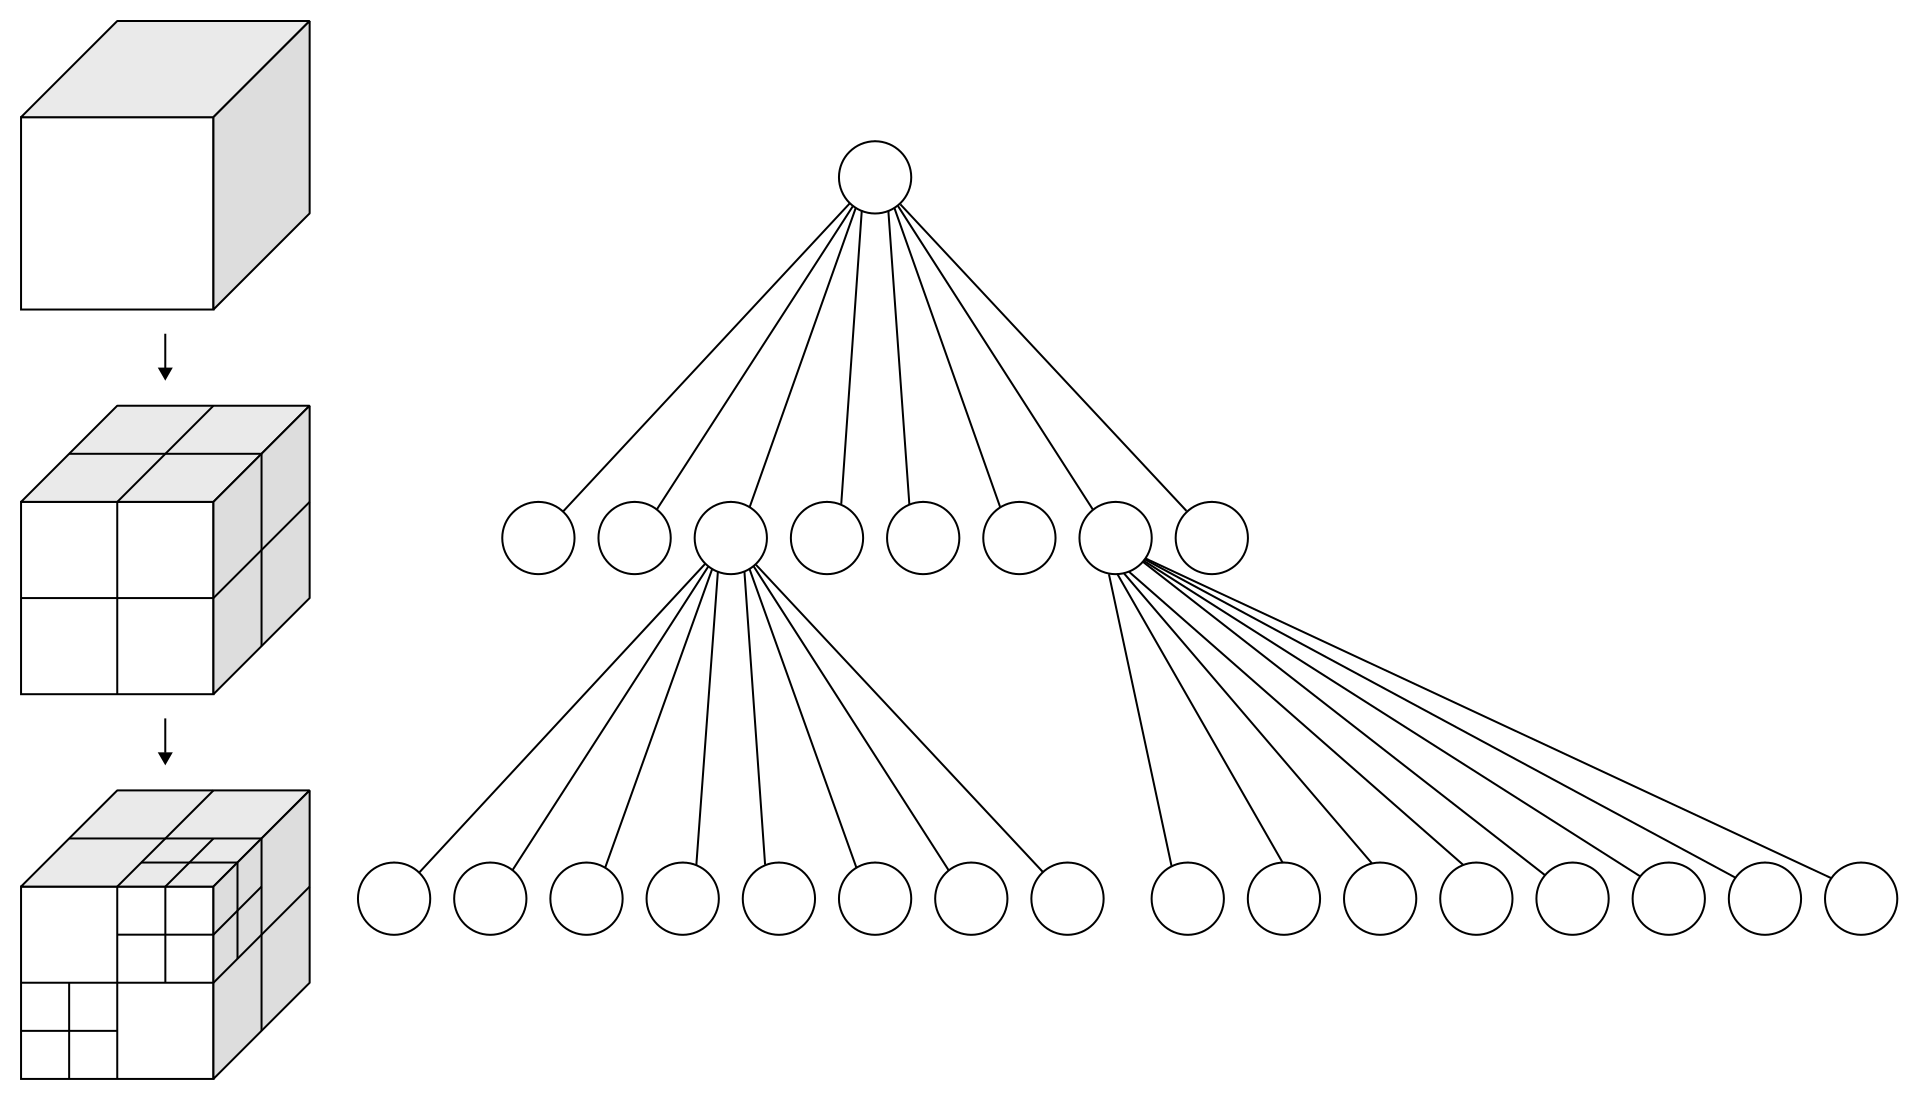
\includegraphics[scale=0.16]{Images/Octree2.svg.png}
    \caption {Octree mesh with level 1 global refinement and level 2 refinement in element2 and 6.}
    \label{fig: octree}
\end{figure}
\\In particular, if we refer to the root of the tree as the element at level 0, we can say that a subelement has level N if it has been obtained by refining the root N times. Analogously, it is possible to coarsen the mesh, aggregating eight octants in order to go back to have only their parent. To every octant we can associate an index, computed following the z-ordering (shown in Figure \ref{fig: z} for a Quadtree), which must be updated after any refinement. To every node of each quadrant are associated two indices: a local index, internal to the quadrant itself, and a global index, related to the position of the node in the full mesh.
\begin{figure}[h!]
    \centering
    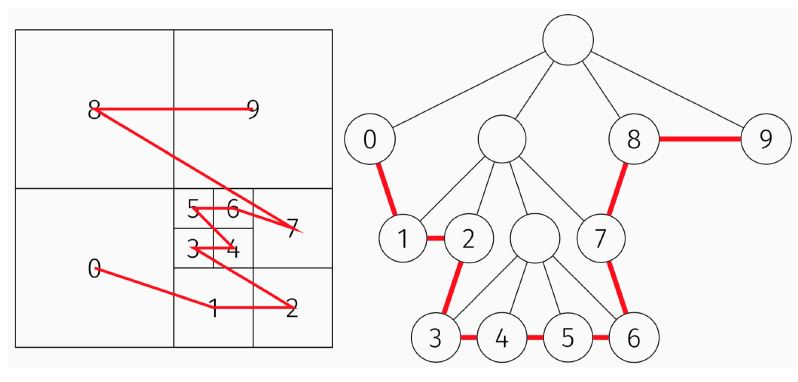
\includegraphics[scale=0.5]{Images/quadtree.JPG}
    \caption {Example of the global numbering for a Quadtree mesh.}
    \label{fig: z}
\end{figure}
\\Each cubic element of the mesh is characterized by the same numbering of faces, edges and nodes, which is the one reported in Figure \ref{fig: enum}.
\begin{figure}[h!]
    \centering
    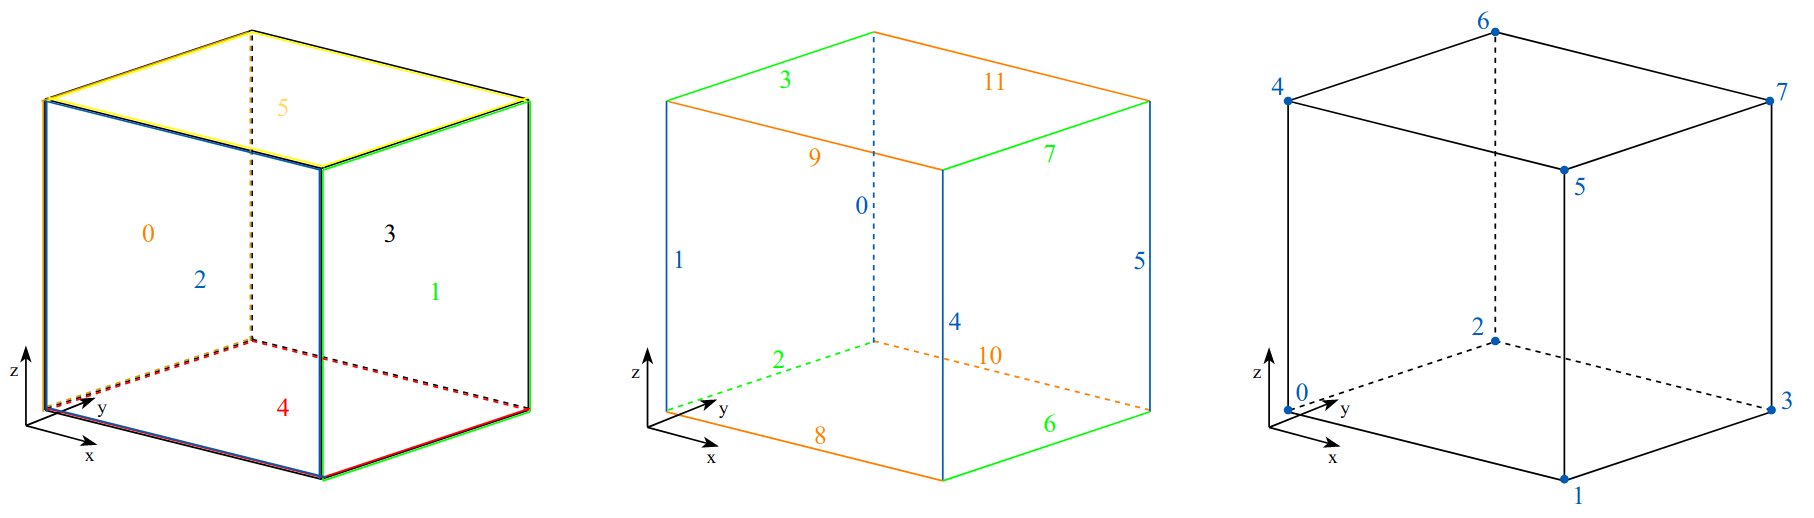
\includegraphics[scale=0.2]{Images/enum}
    \caption {From left to right: numbering of faces, edges, nodes of each quadrant.}
    \label{fig: enum}
\end{figure}
\\The refinement and coarsening processes can lead to hanging nodes, which are nodes lying on an edge which is refined for two elements, but not for the neighboring one (Figure \ref{fig: hanging}).
\begin{figure}[h!]
    \centering
    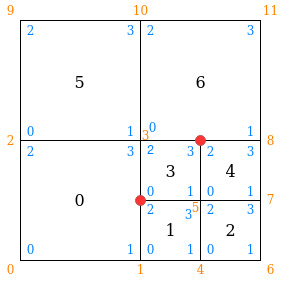
\includegraphics[scale=0.6]{Images/hanging.jpg}
    \caption {Example of hanging nodes for Quadtree mesh. Hanging nodes are marked with red spots, black numbers refer to quadrant numbering, blue to node local indices, orange to node global indices.}
    \label{fig: hanging}
\end{figure}
Hanging nodes have the usual local numbering but they do not have a global numbering, instead they are related to the global numbering of their parents, i.e. to the global numbering of the two non-hanging nodes lying on the same edge.

An Octree mesh is a partition $\tau_h$ of $\Omega$ in $N_h$ elements such that:
\begin{equation}
    \tau_h=\{\Omega^k\}_{k=1}^N,\qquad \Omega_h=\bigcup_{k=1}^N\Omega^k\subseteq \Omega
    \label{eq: partition 1}
\end{equation}
We can now define a space of continuous piecewise tri-linear polynomials $Q^1_h(\tau_h)$ over the given partition $\tau_h$:
\begin{equation}
    Q^1_h(\tau_h)=\left\{u\in C^0(\Bar{\Omega}_h)\ \text{s.t.}\ u|_{\Omega^k}\in\mathbb{P}_{1,1,1}(\Omega^k)\ \forall \Omega^k\in\tau_h\right\}
    \label{eq: partition 2}
\end{equation}
where
\begin{equation}
    \mathbb{P}_{m,n,l}(\Omega)=\{p:\Omega\rightarrow\mathbb{R}\ \text{s.t.}\ p(x,y,z)=\sum_{i\le m,\ k\le n,\ k\le l}a_{ijk}x^iy^jz^k\ \forall (x,y,z)\in\Omega\}
    \label{eq: partition 3}
\end{equation}
Since the Octree mesh can be non-conforming, the space $Q^1_h(\tau_h)$ defined in \ref{eq: partition 2} is not the finite element space used for our solution; however the actual space $\Tilde{Q}^1_h(\Tilde{\tau}_h)$ is a subspace of $\Bar{Q}^1_h(\Bar{\tau}_h)$ if we consider $\Bar{\tau}_h$ to be the mesh obtained with uniform refinement with level equal to the maximum level used in $\Tilde{\tau}_h$. $\Tilde{Q}^1_h(\Tilde{\tau}_h)$ is obtained by modifying the starting space at each refinement and coarsening step.
\\In order to describe the refining procedure, consider the situation where we take an octant form refinement level $N$ to $N+1$. Let $\tau_h$ be the original mesh, $\Tilde{\tau}_h$ the one obtained from the refinement and let $\Bar{\tau}_h$ br the one obtained from an uniform refinement of level $N+1$. Now let $\{\phi_i\}\subset Q^1_h(\tau_h)$, $\{\Tilde{\phi}_i\}\subset \Tilde{Q}^1_h(\Tilde{\tau}_h)$ and $\{\Bar{\phi}_i\}\subset \Bar{Q}^1_h(\Bar{\tau}_h)$ we the corresponding basis. Then, if $\phi_k,\dots,\phi_{k+7}\in Q^1_h(\tau_h)$ are the basis elements for the vertex of the considered element and $\Bar{\phi}_{k+8}\in\Bar{Q}^1_h(\Bar{\tau}_h)$ is the basis element for the newly created vertex at the centre of the element, then we can define
\begin{equation}
    \Tilde{\phi}_{k+i}=\phi_{k+i}-\frac{1}{8}\Bar{\phi}_{k+8}\quad\forall i=0,\dots,7
    \label{eq: refinement}
\end{equation}
The other basis elements of $\Tilde{Q}^1_h(\Tilde{\tau}_h)$ are the same of $Q^1_h(\tau_h)$, plus the addition of $\Bar{\phi}_{k+8}$. Note that $\Tilde{Q}^1_h(\Tilde{\tau}_h)\subset\Bar{Q}^1_h(\Bar{\tau}_h)$. Moreover, its basis function still satisfy:
\begin{equation}
    \sum_i \Tilde{\phi}_{i}=1,\qquad \Tilde{\phi}_{i}(x_j)=\delta_{ij}\quad \forall x_j\in \Tilde{X} 
    \label{eq: refinement 2}
\end{equation}
where $\Tilde{X}$ is the set of nodes defining $\Tilde{\tau}_h$.

Coarsening is performed in a similar fashion, by adding a fraction of the deleted basis $\phi_k$ function to the surround ones in order to maintain the partition of unity property. If $\Tilde{\phi}_i$ are the resulting basis functions defined on the vertices of the octant after the coarsening, we have:
\begin{equation}
    \Tilde{\phi}_{i}=\phi_{i}+\frac{1}{2}\sum_{j\in M_i^B}\phi_j+\frac{1}{4}\sum_{j\in M_i^F}\phi_j+\frac{1}{8}\phi_k
    \label{eq: coarsening}
\end{equation}
where $M_i^B$ is the set of nodes that share an edge with node $k$ and $M_i^F$ is the set of
nodes that share a face with node $k$.

\chapter{bim++ library}
The bim++ library is an interface to p4est (and its 3D version p8est), the dynamic back-end manager of quadtree (octree). It is an efficient, parallel, scalable finite element code that allows to solve advection-diffusion-reaction problem.

\section{Quadtree/Octree}
\label{ch: octree}%
The first step is to define the mesh object using the class tmesh\_3d.
\begin{lstlisting}[language=C++]
tmesh_3d tmsh;
tmsh.read_connectivity (simple_conn_p, simple_conn_num_vertices,
                          simple_conn_t, simple_conn_num_trees);
\end{lstlisting}
We then import the connectivity, which consists of the nodes and coordinates of the vertex of our cube.
\begin{lstlisting}[language=C++]
constexpr p4est_topidx_t simple_conn_num_vertices = 8;
constexpr p4est_topidx_t simple_conn_num_trees = 1;
const double simple_conn_p[simple_conn_num_vertices*3] = 
  {0., 0., 0., 0.001, 0., 0., 0., 0.001, 0., 0.001, 0.001, 0.,
   0., 0., 0.001, 0.001, 0., 0.001, 0., 0.001, 0.001, 0.001, 0.001, 0.001};
const p4est_topidx_t simple_conn_t[simple_conn_num_trees*9] = 
  {1, 2, 3, 4, 5, 6, 7, 8, 1};
\end{lstlisting}
Here is an example of refinement function, which assign a value greater that zero to each octant which has to be refined, zero otherwise.
\begin{lstlisting}[language=C++]
static int
ball_refinement (tmesh_3d::quadrant_iterator quadrant)
{
  int currentlevel = static_cast<int> (quadrant->the_quadrant->level);
  double xcoord, ycoord, zcoord, dist = .0;
  int retval = 0;
  for (int ii = 0; ii < 8; ++ii)
    {
      xcoord = quadrant->p(0, ii);
      ycoord = quadrant->p(1, ii);
      zcoord = quadrant->p(2, ii);
      
      dist = std::sqrt (std::pow (xcoord - b_x, 2) +
                        std::pow (ycoord - b_y, 2) +
                        std::pow (zcoord - b_z, 2));
      if (dist < 1.1 * b_r)
        {
          retval = maxlevel_ball - currentlevel;
          break;
        }
    }
  if (currentlevel >= maxlevel_ball)
    retval = 0;
      
  return (retval);
}
\end{lstlisting}

We finally perform uniform and non-uniform refinement
\begin{lstlisting}[language=C++]
int recursive = 1;
tmsh.set_refine_marker (uniform_refinement);
tmsh.refine (recursive);

tmsh.set_refine_marker(ball_refinement);
tmsh.refine (recursive);
\end{lstlisting}

\section{Assembly}
We first define the orderings, which allow us to differentiate between the two unknowns $\phi$ and $\rho$ is the solution vector. They also identify which rows of the system matrix correspond to which equation in our linear system.
\begin{lstlisting}[language=C++]
ord0 = [] (tmesh_3d::idx_t gt) -> size_t { return dof_ordering<2, 0> (gt); },
ord1 = [] (tmesh_3d::idx_t gt) -> size_t { return dof_ordering<2, 1> (gt); };
\end{lstlisting}
The following lines assemble in the matrix "A" the part related to the diffusion of $\phi$: $-\nabla\cdot(\epsilon_0\epsilon_\infty\nabla\phi)$ for the first equation and $-\nabla\cdot(\Delta t\sigma\nabla\phi)$ for the second.
\begin{lstlisting}[language=C++]
// advection_diffusion
bim3a_advection_diffusion (tmsh, epsilon, zero, A, true, ord0, ord0);
bim3a_advection_diffusion (tmsh, sigma, zero, A, true, ord1, ord0);
\end{lstlisting}
These lines assemble in the matrix "A" the part related to the reaction term $-\rho$ in the first equation and $\rho$ in the second.
\begin{lstlisting}[language=C++]
// reaction
bim3a_reaction (tmsh, delta0, zeta0, A, ord0, ord1);
bim3a_reaction (tmsh, delta1, zeta1, A, ord1, ord1);
\end{lstlisting}
The homogeneues and non-homogeneus time-dependent boundary conditions are set up and implemented for the variable $\phi$.
\begin{lstlisting}[language=C++]
dirichlet_bcs3 bcs0;
    
bcs0.push_back (std::make_tuple (0, 4, [](double x, double y, double z){return 0.0;})); //bottom
bcs0.push_back (std::make_tuple (0, 5, [time](double x, double y, double z){return 1.5e4 * (1 - exp(-tau/10.0));})); //top
    
bim3a_dirichlet_bc_bis (tmsh, bcs0, A, sol, ord1, ord0, false);
\end{lstlisting}
Since this was the first case of system of differential equation in three dimensions in bim++ with dirichlet boundary conditions on one variable only, the following functions needed to be implemented. 
\begin{lstlisting}[language=C++]
template <class T>
void
bim3a_dirichlet_bc (tmesh_3d& mesh, const dirichlet_bcs3& bcs,
                    sparse_matrix& A, T& rhs,
                    const ordering& ordr,
                    const ordering& ordc,
                    const bool& only_rhs)
{
  int boundary_idx, tree_idx;
  unsigned int row, col;

  std::set<unsigned int> marked;

  double value;

  for (auto quadrant = mesh.begin_quadrant_sweep ();
       quadrant != mesh.end_quadrant_sweep ();
       ++quadrant)
    {
      tree_idx = quadrant->get_tree_idx ();

      for (int i = 0; i < 8; ++i)
        {
          boundary_idx = quadrant->e (i);
          row = ordr (quadrant->gt (i));
          col = ordc (quadrant->gt (i));

          // If current node is on boundary and has not
          // been handled before.
          if (boundary_idx != tmesh_3d::quadrant_t::NOT_ON_BOUNDARY
              && marked.count(row) == 0)
            {
              // Loop over all the boundary conditions.
              for (size_t bc = 0; bc < bcs.size (); ++bc)
                // If this boundary condition matches with
                // the current node.
                if (std::get<0> (bcs[bc]) == tree_idx
                    && std::get<1> (bcs[bc]) == boundary_idx)
                  {
                    // Mark current node so to avoid duplicate operations.
                    marked.insert (row);

                    // Evaluate bc at current node
                    value = (std::get<2> (bcs[bc]))
                            (quadrant->p (0, i),
                              quadrant->p (1, i),
                              quadrant->p (2, i));

                    bim3a_dirichlet_bc_loc (A, rhs, row, col, value, only_rhs);
                  }
            }
        }
    }
}
\end{lstlisting}
\begin{lstlisting}[language=C++]
template <class T>
void
bim3a_dirichlet_bc_loc (sparse_matrix& A,
                        T& rhs,
                        const unsigned int& row,
                        const unsigned int& col,
                        const double& value,
                        const bool& only_rhs)
{
  if (std::abs (A[row][col]) < std::numeric_limits<double>::epsilon())
    {
      A[row][col] = std::accumulate
        (A[row].begin (),
         A[row].end (),
         0.0,
         [] (double sum,
             const std::map<int, double>::value_type & p)
         {
           return (sum + std::abs (p.second));
         }
         );
    }

  if (! only_rhs)
    A[row][col] *= 1e16;

  // Multiply rhs by the diagonal entry
  rhs[row] = A[row][col] * value;
}
\end{lstlisting}
Finally, the right-hand-side vector \textit{sol} is assembled at each time step since it depends on the values of $\rho$ at the previous time step. 
\begin{lstlisting}[language=C++]
for (auto quadrant = tmsh.begin_quadrant_sweep (); quadrant != tmsh.end_quadrant_sweep (); ++quadrant)
{
    for (int ii = 0; ii < 8; ++ii)
        if (! quadrant->is_hanging (ii))
            g1[quadrant->gt (ii)] = sold[ord1(quadrant->gt (ii))];
          
        else
            for (int jj = 0; jj < quadrant->num_parents (ii); ++jj)
                g1[quadrant->gparent (jj, ii)] += 0.;
}
    
//rhs
bim3a_rhs (tmsh, f0, g0, sol, ord0);
bim3a_rhs (tmsh, f1, g1, sol, ord1);
\end{lstlisting}
\section{Linear solver}
The library we use to solve our linear system is MUMPS \cite{MUMPS} (“MUltifrontal Massively Parallel Solver”), which is a package for solving systems of linear equations of the form $\bm{A}x = b$, where $\bm{A}$ is a square sparse matrix that can be either unsymmetric, symmetric positive definite, or general symmetric, on distributed memory computers. MUMPS implements a direct method based on a multifrontal approach which performs a Gaussian factorization $\bm{A} = \bm{L}\bm{U}$,
where $\bm{L}$ is a lower triangular matrix and $\bm{U}$ an upper triangular matrix. If the matrix is symmetric then the factorization $\bm{A} = \bm{L}\bm{D}\bm{L}^T$, where $\bm{D}$ is block diagonal matrix, is performed.
\\The system $\bm{A}x = b$ is solved in three main steps:
\begin{enumerate}
    \item Analysis, during which preprocessing, including an ordering based on the symmetrized pattern $\bm{A}+\bm{A}^T$, and a symbolic factorization are performed.
    \item Factorization, during which $\bm{A}_\text{pre} = \bm{L}\bm{U}$ or $\bm{A}_{pre} = \bm{L}\bm{D}\bm{L}^T$, depending on the symmetry of the preprocessed matrix, is computed.
    \item Solution, where the solution vector $x_\text{pre}$ of $\bm{L}\bm{U}x_\text{pre} = b_{pre}$ or $\bm{L}\bm{D}\bm{L}^T x_\text{pre} = b_\text{pre}$ is obtained through a forward elimination step $\bm{L}y = b_\text{pre}$ or $\bm{L}\bm{D}y = b_\text{pre}$, followed by a backward elimination step $\bm{U}x_\text{pre} = y$ or $\bm{L}^Tx_\text{pre} = y$. $x_\text{pre}$ and $b_\text{pre}$ are respectively the transformed solution $x$ and right-hand side $b$ associated to the preprocessed matrix $\bm{A}_\text{pre}$, 
\end{enumerate}
\begin{lstlisting}[language=C++]
// Communicate matrix and RHS
A.assemble ();
sol.assemble ();

// Solver analysis
lin_solver->set_lhs_distributed ();
A.aij (xa, ir, jc, lin_solver->get_index_base ());
lin_solver->set_distributed_lhs_structure (A.rows (), ir, jc);
std::cout << "lin_solver->analyze () return value = "<< lin_solver->analyze () << std::endl;

// Matrix update
A.aij_update (xa, ir, jc, lin_solver->get_index_base ());
    lin_solver->set_distributed_lhs_data (xa);

// Factorization
std::cout << "lin_solver->factorize () = " << lin_solver->factorize () << std::endl;

// Set RHS data
lin_solver->set_rhs_distributed (sol);

// Solution
std::cout << "lin_solver->solve () = " << lin_solver->solve () << std::endl;
\end{lstlisting}

\section{Using the library}
We report here the instruction to use the library, see the file \textit{README.md} for more details.
\\In the main file \textit{HVDC\_main.cpp}, choose one of the tests by including the appropriate header file at lines 32-36. Then, compile the code with 
\begin{lstlisting}[language=bash]
make all
\end{lstlisting}
\\To generate the Doxygen documentation, run the command 
\begin{lstlisting}[language=bash]
make doc
\end{lstlisting}
Only the main file \textit{HVDC\_main.cpp} and the header file \textit{Test\_3.h} are included, the other header files have a similar structure so they are omitted.
\\The post processing is performed with two Octave functions included in the \textit{script/m} folder. The first one, \textit{export\_phi\_rho.m}, requires the function \textit{export\_tmesh\_data.m} provided with bim++, so it is necessary to add the path \textit{script/m} of bim++ to the Octave path. It generates the .vtu files, which can by opened using Paraview. The usage is the following:
\begin{lstlisting}[language=octave]
export_phi_rho(<final time step>, <number of processes>)
\end{lstlisting}
with \textit{final time step} being the index of the last time step and \textit{number of processes} equal to the used number of processors. 
\\Moreover, the file \textit{rho.m} contains a function that generates a plot of the value of the charge density rho over time at the points specified in the .h file. The usage is the following:
\begin{lstlisting}[language=octave]
rho(<refinement levels>,<cube side length>=0.001)
\end{lstlisting}
where \textit{refinement levels} is a vector with the refinement levels of at the nodes selected by the \textit{rho\_idx} variable, and \textit{cube side length} is the cubic domain dimension.


\chapter{Numerical Results}
The following tests will be performed with the level 0 model \ref{eq: m0 time} and the following values for some of the parameters:
\[L=0.001,\quad V_0=15kV,\ \sigma=3.21e-14\quad \epsilon_0=8.8542e-12\]
and as boundary condition we take \ref{eq: bc}.
\section{Test 1}
In the first test we consider a uniform value for permittivity equal to $\epsilon=\epsilon_r\epsilon_0$, with $\epsilon_r=2$. The mesh has a uniform refinement of level $N_\text{ref}=4$ as shown in Figure \ref{fig: 1.1}.
The other parameters are set to $T=15,\ \Delta t=0.1,\ \tau=2.0$.
\begin{figure}[h!]
    \centering
   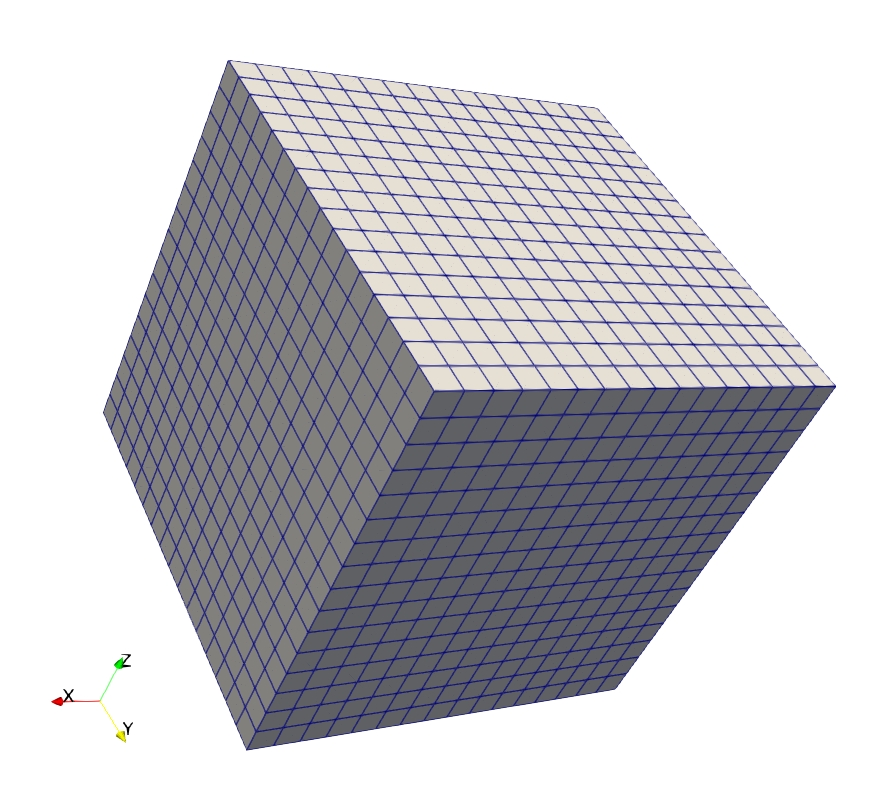
\includegraphics[scale=0.25]{Images/1.grid.jpeg}
    \caption {Test 1: uniform mesh, $N_\text{ref}=4$.}
    \label{fig: 1.1}
\end{figure}
\\The potential is uniform along the x and y axes, and it has a uniform gradient along the z axes (Figure \ref{fig: 1.2}).
\begin{figure}[h!]
    \centering
   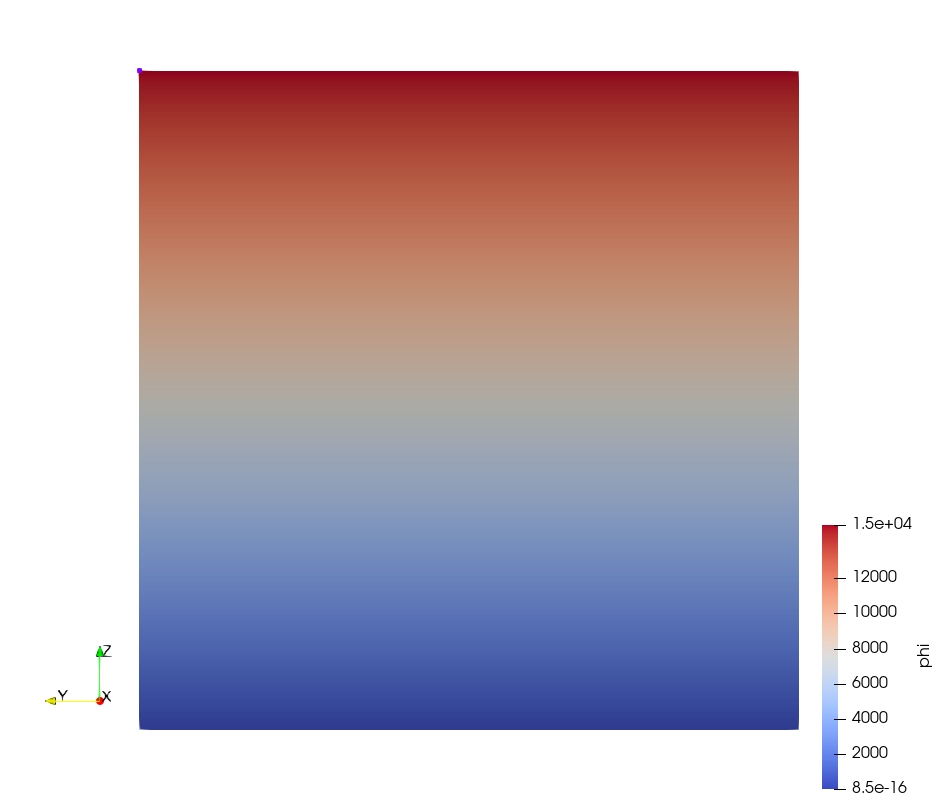
\includegraphics[scale=0.2]{Images/1.pot_3d.jpeg}
   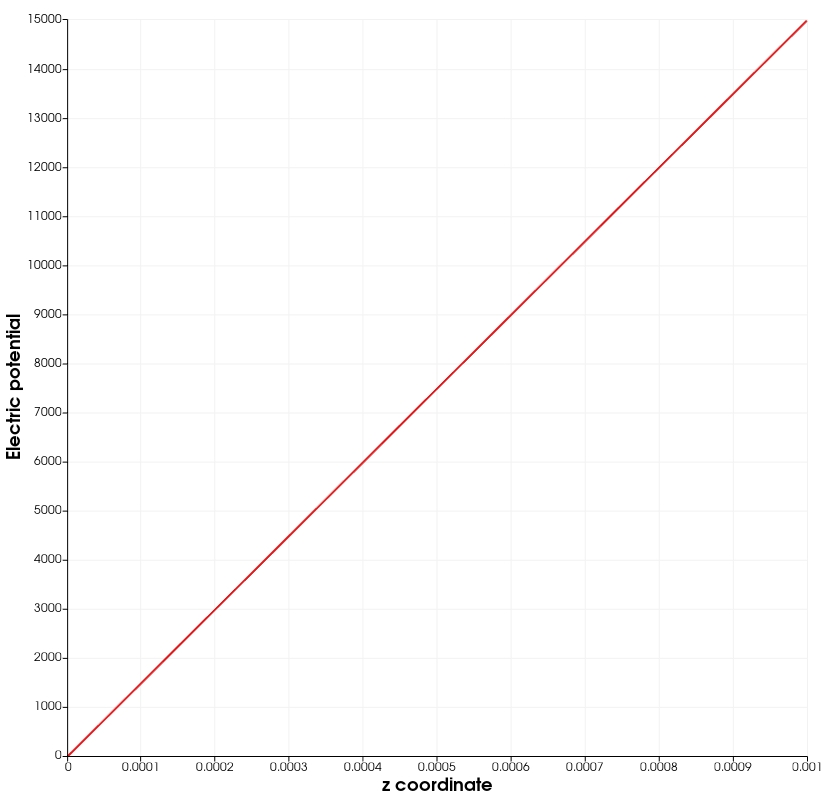
\includegraphics[scale=0.2]{Images/1.pot.jpeg}
    \caption {Test 1: electric potential in the cube (left) and as a function of the z coordinate (right) for $t=T$.}
    \label{fig: 1.2}
\end{figure}
\\We have an accumulation of positive charge on the top face and of negative charge on the bottom face, again uniform along the x and y axes, whereas in the remaining part of the domain the charge is zero (Figure \ref{fig: 1.3}).
\begin{figure}[h!]
    \centering
   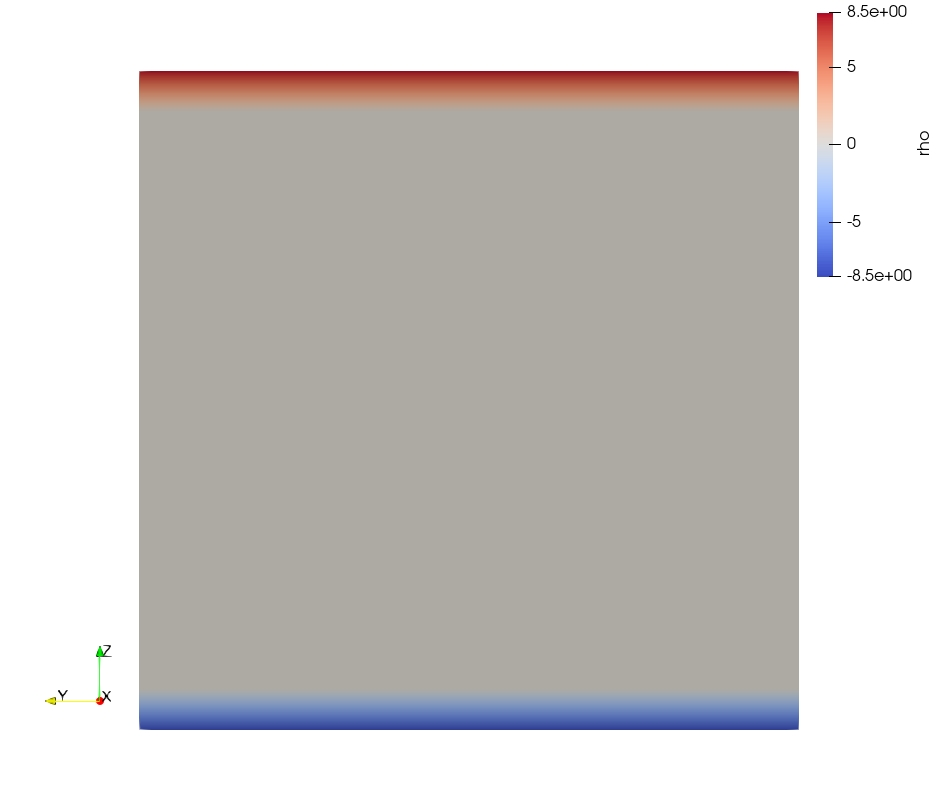
\includegraphics[scale=0.2]{Images/1.rho_3d.jpeg}
   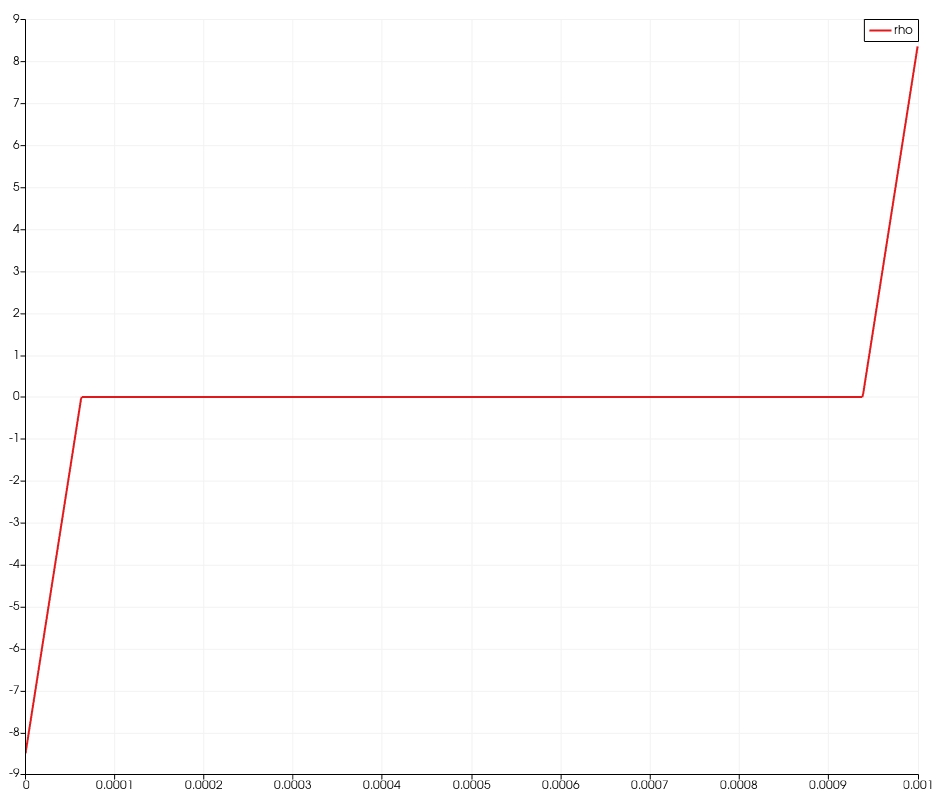
\includegraphics[scale=0.2]{Images/1.rho.jpeg}
    \caption {Test 1: charge density in the cube (left) and as a function of the z coordinate (right) for $t=T$.}
    \label{fig: 1.3}
\end{figure}
\\The charge accumulation over time follows an asymptotic exponential behaviour with time constant equal to $\tau$, as shown in Figure \ref{fig: 1.4}.
\begin{figure}[h!]
    \centering
   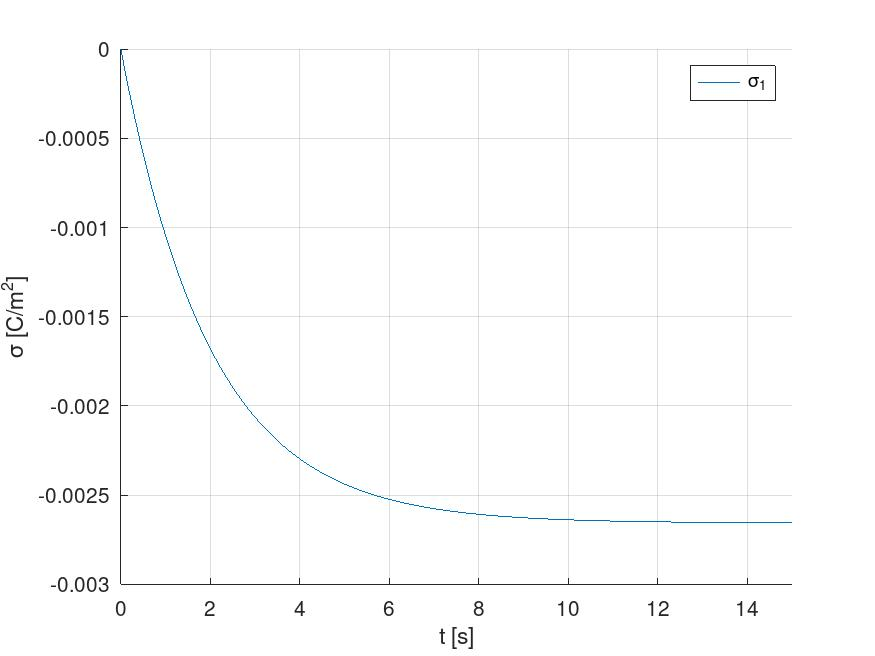
\includegraphics[scale=0.2]{Images/1.rho_time.jpeg}
    \caption {Test 1: charge density in the bottom face as a function of time.}
    \label{fig: 1.4}
\end{figure}

\section{Test 2}
In the second test we consider two values for the permittivity: $\epsilon_r=2$ for $z<0.0005$ and $\epsilon_r=4$ otherwise.
The mesh has a uniform refinement of level $N_\text{ref}=4$ plus a local refinement of level $N_\text{ref,loc}=7$ along the plane $z=0.0005$, see Figure \ref{fig: 2.1}.
\begin{figure}[h!]
    \centering
   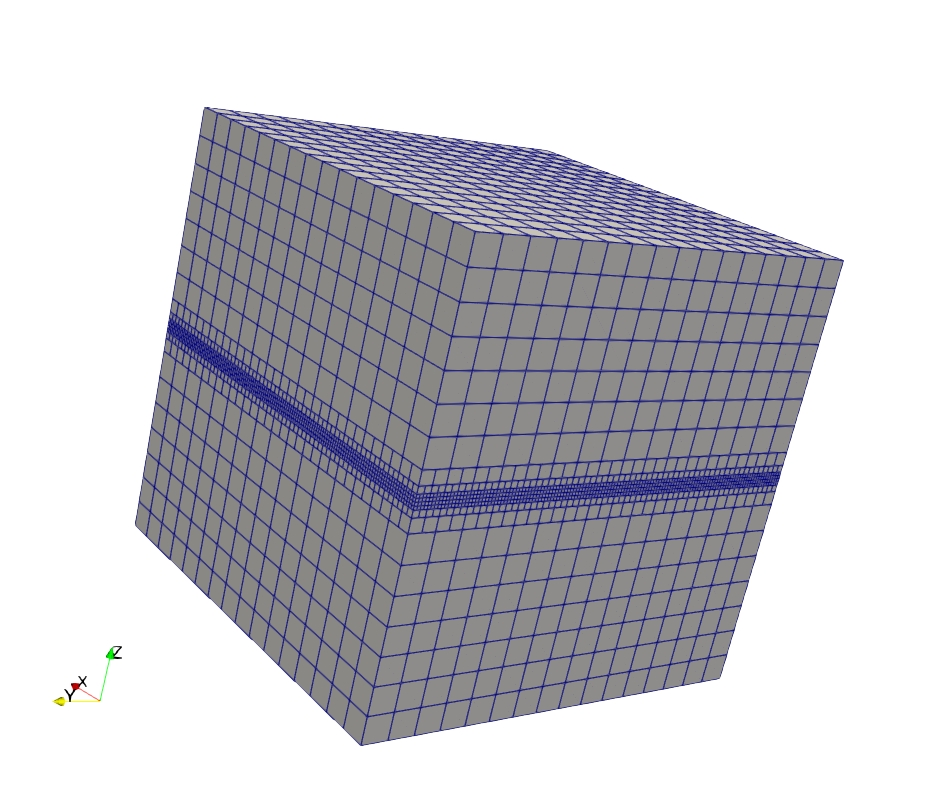
\includegraphics[scale=0.25]{Images/2.grid.jpeg}
    \caption {Test 2: uniform mesh, $N_\text{ref}=4$, with local refinement $N_\text{ref,loc}=6$ at $z=0.0005$.}
    \label{fig: 2.1}
\end{figure}
\\The resulting electric field is identical to the one obtained in Test 1, shown in Figure \ref{fig: 1.2}. 
\\At equilibrium, we have an accumulation of negative charge at the interface (Figure \ref{fig: 2.2}) as expected from theory \cite{charge}.
\begin{figure}[h!]
    \centering
   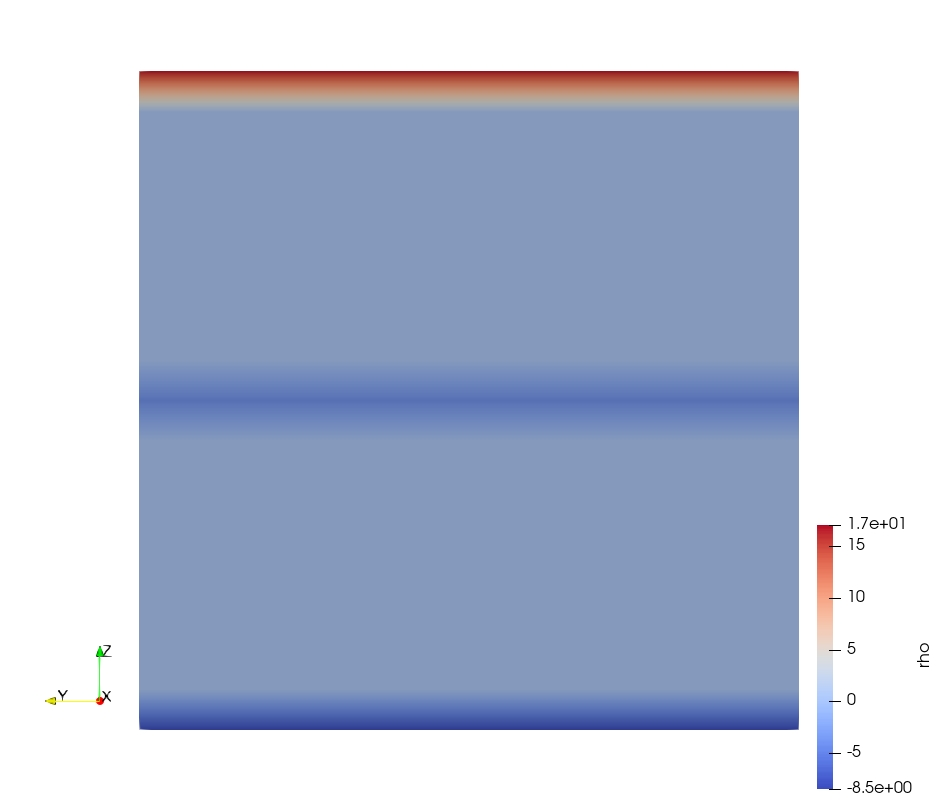
\includegraphics[scale=0.2]{Images/2.rho_3d.jpeg}
   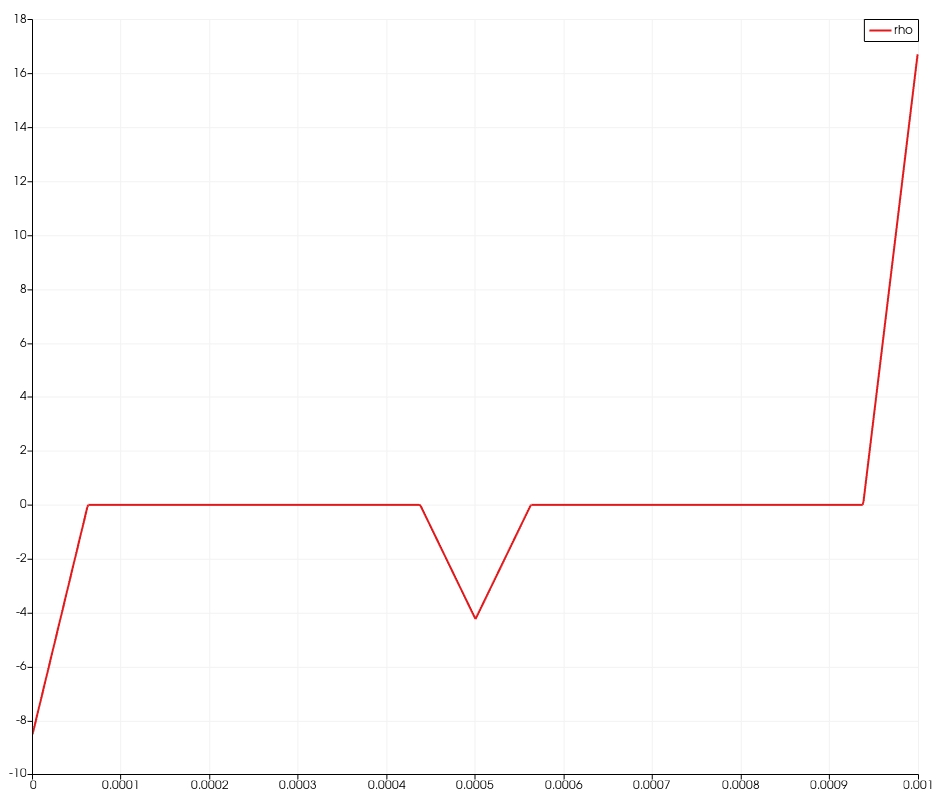
\includegraphics[scale=0.2]{Images/2.rho.jpeg}
    \caption {Test 2: charge density in the cube (left) and as a function of the z coordinate (right) for $t=T$.}
    \label{fig: 2.2}
\end{figure}
\\Note the values of the plots of the type shown in Figure \ref{fig: 2.2} depends on the local refinement level, meaning that the smaller is the grid element, the higher is the shown $\rho$ value compared with a bigger element with the same charge density.
\\The time scale at which the charge accumulates varies significantly: we have first a fast charge accumulation at the conductor interfaces, represented by $\sigma_1$ and $\sigma_3$ in Figure \ref{fig: 2.3} left, followed by a slower movement of charge towards the interface at $z=0.0005$ represented by $\sigma_2$ in Figure \ref{fig: 2.3} right.
\begin{figure}[h!]
    \centering
   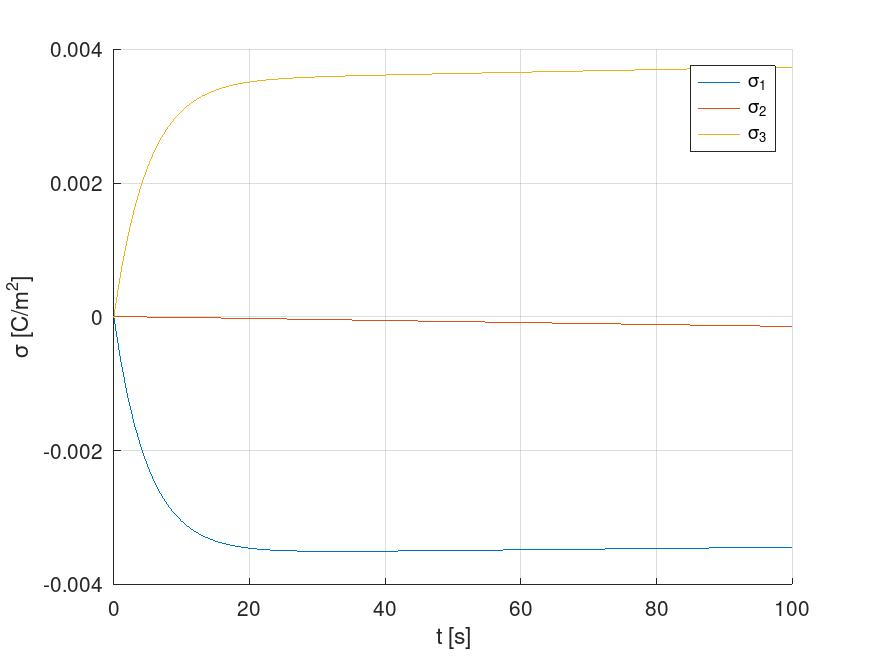
\includegraphics[scale=0.2]{Images/2.rho_time_fast.jpeg}
   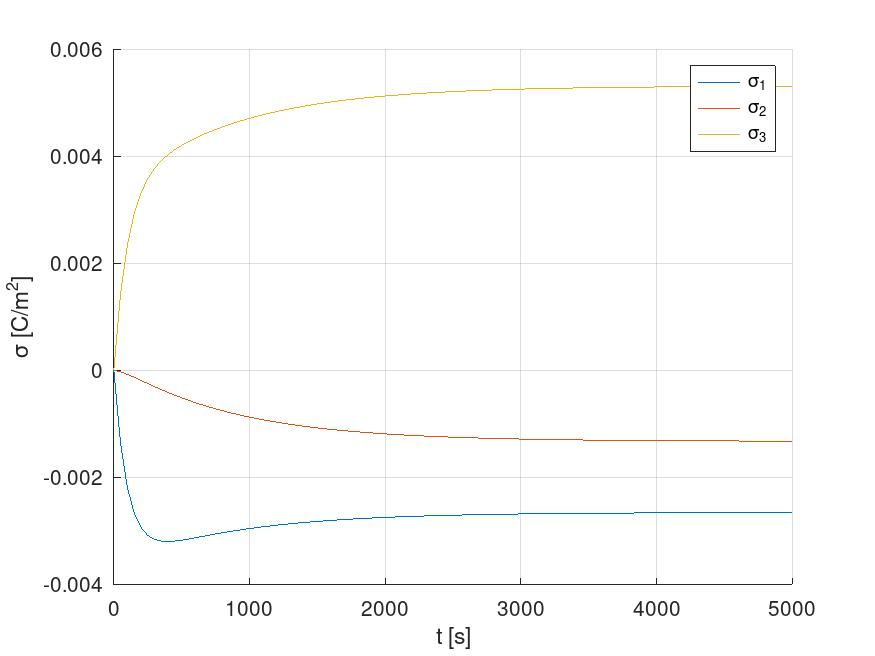
\includegraphics[scale=0.2]{Images/2.rho_time.jpeg}
    \caption {Test 2: charge density as a function of time: the left plot is computed with parameters $T=100,\ \Delta t=1,\ \tau=5$, the right one with $T=5000,\ \Delta t=50,\ \tau=50$. $\sigma_1$ represents the lower interface, $\sigma_2$ represents the central interface and $\sigma_1$ represents the upper interface.}
    \label{fig: 2.3}
\end{figure}

\section{Test 3}
In Test 3 we try to simulate the behaviour of the insulator in mass impregnated cables, represented in Figure \ref{fig: 3.1}. 
\begin{figure}[h!]
    \centering
   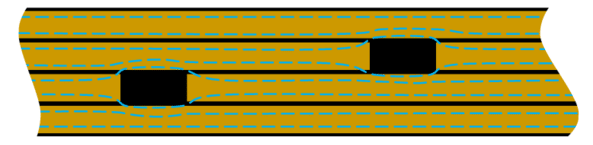
\includegraphics[scale=0.5]{Images/3.butt.png}
    \caption {Test 3: structure of the insulation in a mass impregnated cable (credits: \cite{butt}).}
    \label{fig: 3.1}
\end{figure}
\\We consider a cubic domain with three paper layers alternated by two oil layers, with the paper layer being 6 times thicker than the oil one. Moreover, we insert in the middle paper layer a cubic cavity, usually referred to as a butt-gap, filled with oil. The permittivity for the paper is $\epsilon_r=4$ and for the oil $\epsilon_r=2$.
The mesh has refinement of level $N_\text{ref.loc}=6$ at the interfaces between paper and oil, and $N_\text{ref}=4$ elsewhere (Figure \ref{fig: 3.2}).
\begin{figure}[h!]
    \centering
   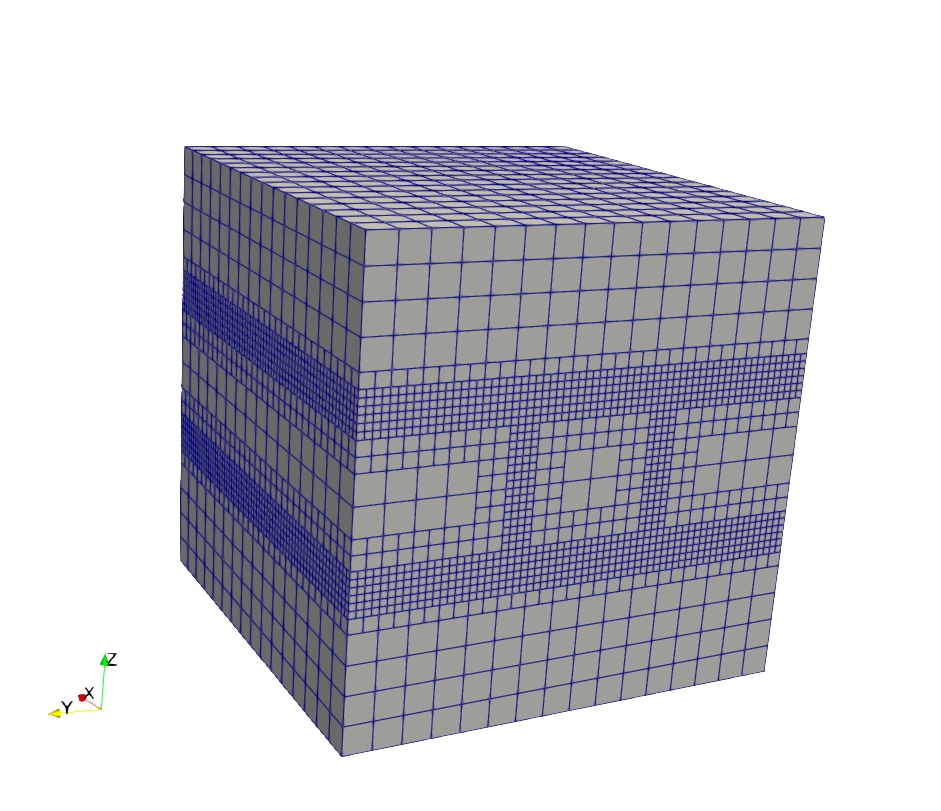
\includegraphics[scale=0.25]{Images/3.grid.jpeg}
    \caption {Test 3: mesh with local refinement of level $N_\text{ref}=6$ at the paper-oil interfaces and at the border of the butt-gap, $N_\text{ref}=4$ elsewhere.}
    \label{fig: 3.2}
\end{figure}
\\The resulting electric field is identical to the one obtained in Test 1, shown in Figure \ref{fig: 1.2}. 
The charge density is shown in figure Figure \ref{fig: 3.3}: we have an accumulation of charges at each interface, but not near the butt-gap since it oil filled and it is in contact with two oil layers. We don't have accumulation on the vertical faces of the butt-gap.
\begin{figure}[h!]
    \centering
   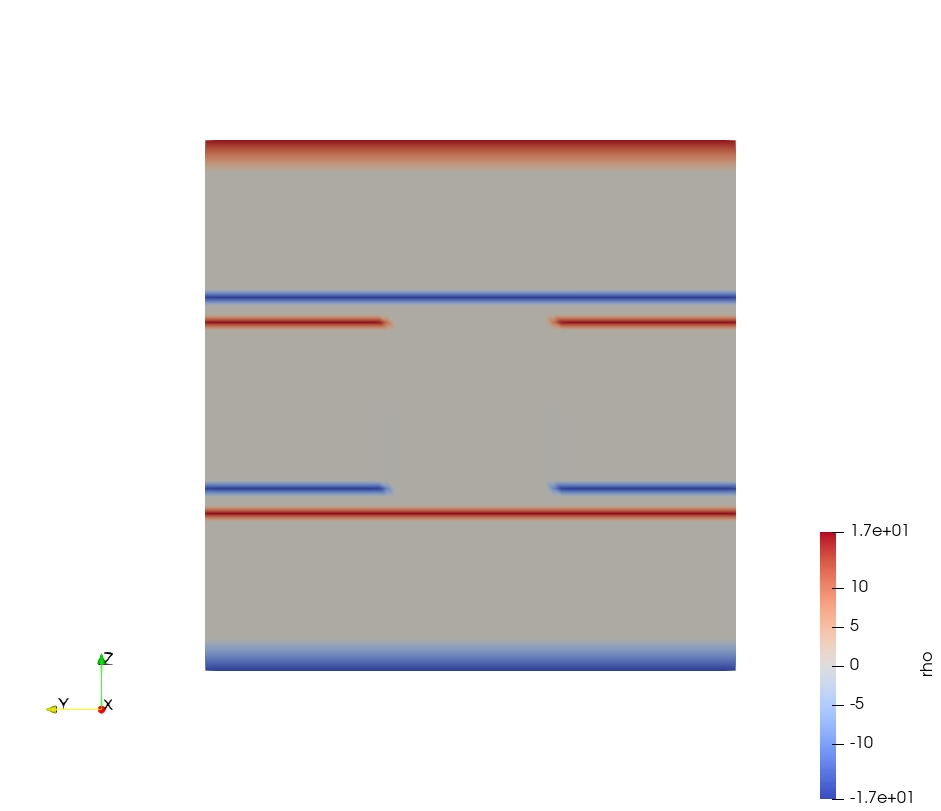
\includegraphics[scale=0.2]{Images/3.rho_3d.jpeg}
   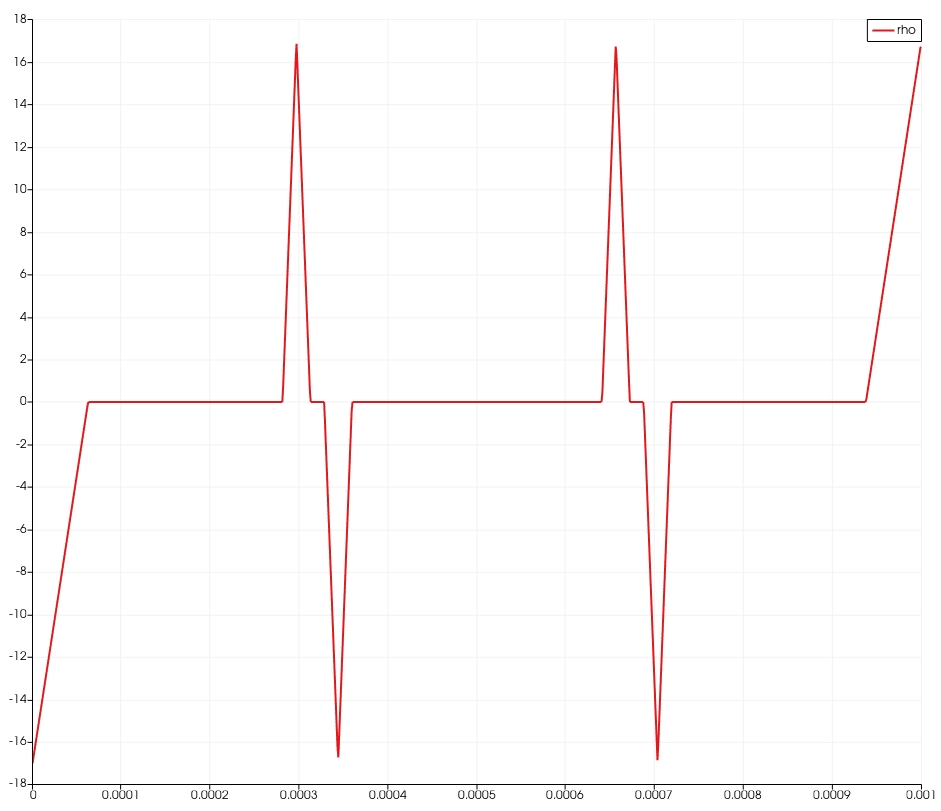
\includegraphics[scale=0.2]{Images/3.rho.jpeg}
    \caption {Test 3: charge density in the cube (left) and as a function of the z coordinate (right) for $t=T$.}
    \label{fig: 3.3}
\end{figure}
\\In Figure \ref{fig: 3.4} we represent the charge values at different points over time. As before, the charge quickly accumulate on the top and bottom faces ($\sigma_1$ and $\sigma_6$), and then more slowly accumulates on the internal paper-oil interfaces.
\begin{figure}[h!]
    \centering
   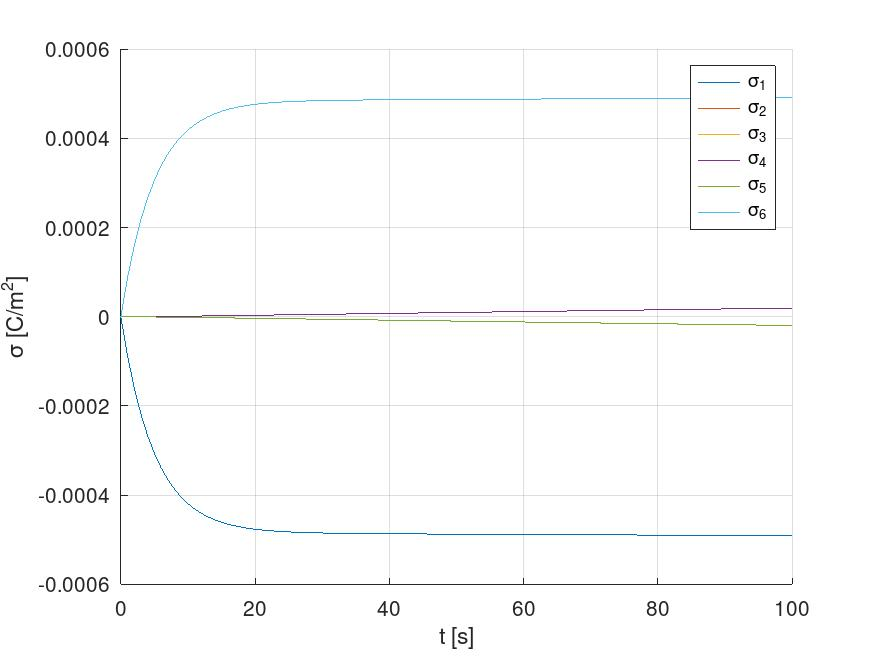
\includegraphics[scale=0.2]{Images/3.rho_time_fast.jpeg}
   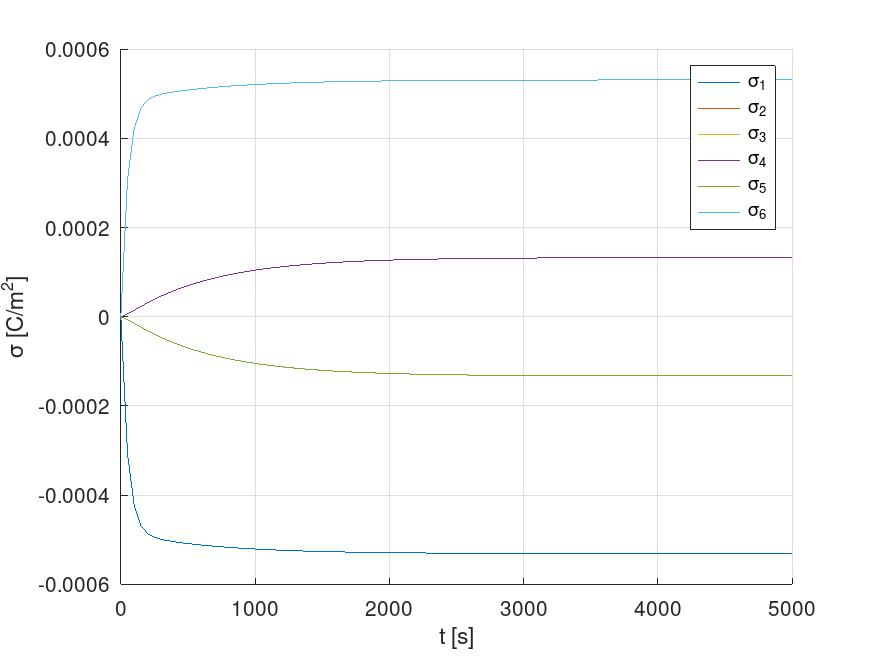
\includegraphics[scale=0.2]{Images/3.rho_time.jpeg}
    \caption {Test 3: charge density as a function of time: the left plot is computed with parameters $T=100,\ \Delta t=1,\ \tau=5$, the right one with $T=5000,\ \Delta t=50,\ \tau=50$. $\sigma_1$ represents the lower interface, $\sigma_2$ the first paper-oil interface, $\sigma_3$ the first oil-paper interface, $\sigma_4$ and $\sigma_5$ the second paper-oil and oil-paper interfaces and $\sigma_6$ represents the upper interface. Note that the plot for $\sigma_2$ overlaps with $\sigma_4$ and $\sigma_3$ with $\sigma_5$.}
    \label{fig: 3.4}
\end{figure}


\section{Test 4}
In Test 4 we consider an analogous scenario to Test 3, but this time the butt-gaps are filled with air, which we consider to have a permittivity value $\epsilon_r=1$ and conductivity $\sigma=1e-12$
\begin{figure}[h!]
    \centering
   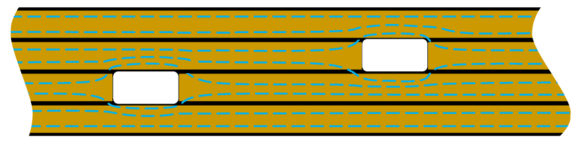
\includegraphics[scale=0.5]{Images/4.butt.png}
    \caption {Test 4: structure of the insulation in a mass impregnated cable (credits: \cite{butt}).}
    \label{fig: 4.1}
\end{figure}
\\The mesh is identical to the one used in Test 3. The electric field shows a sharp change in slope in the air filled butt-gap as shown in Figure \ref{fig: 4.1.5}.
\begin{figure}[h!]
    \centering
   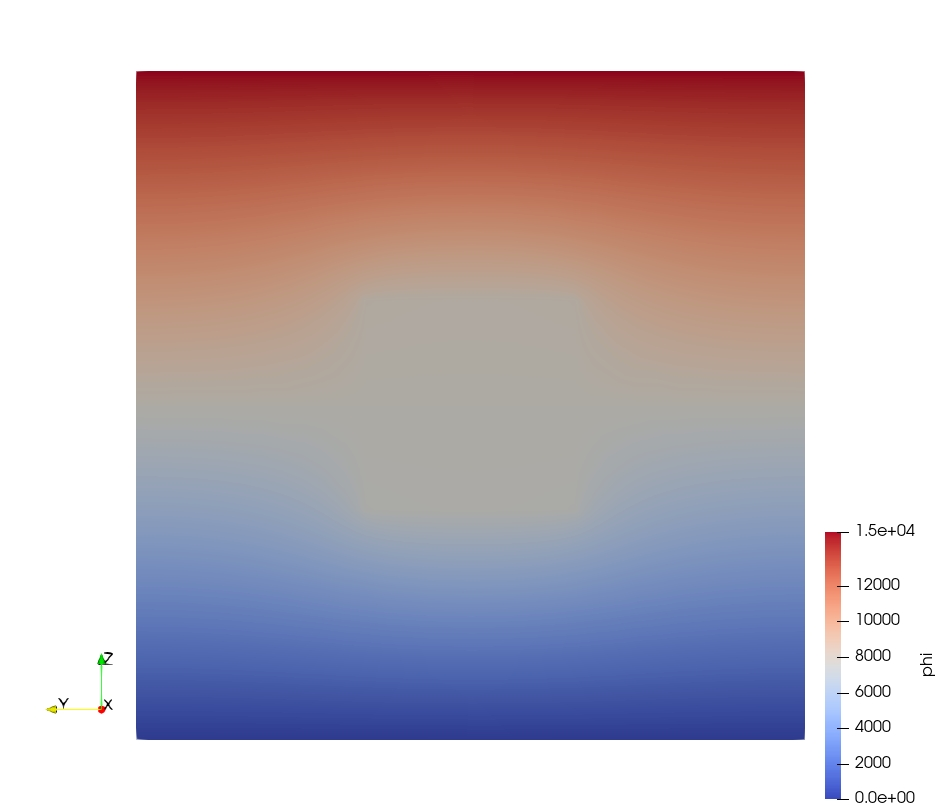
\includegraphics[scale=0.2]{Images/4.phi_3d.jpeg}
   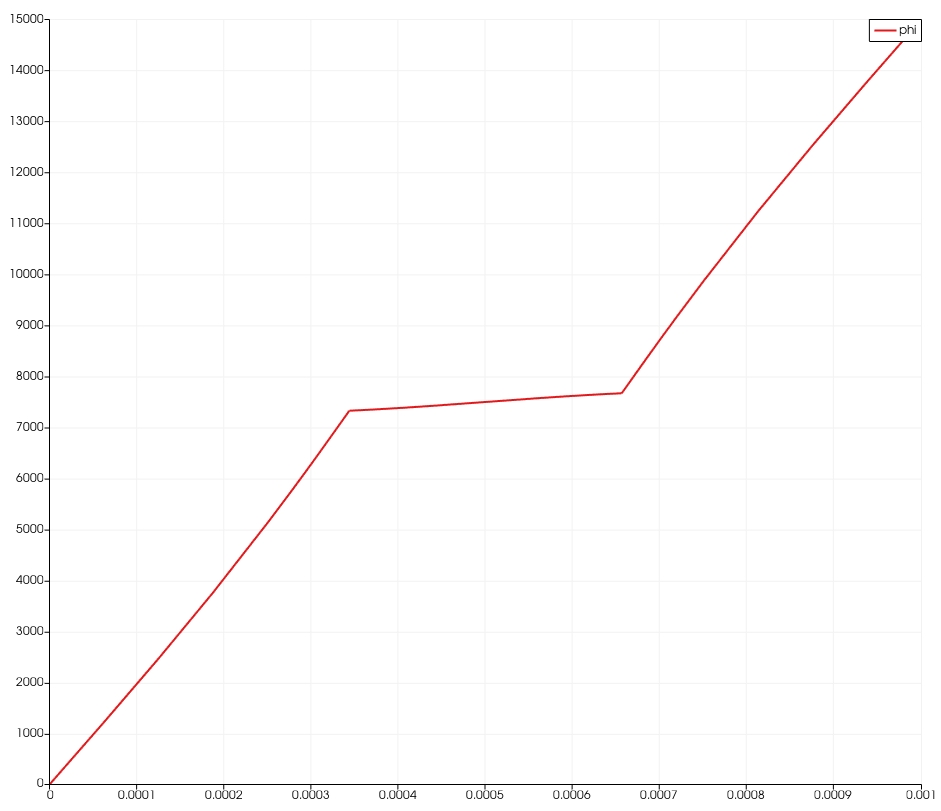
\includegraphics[scale=0.2]{Images/4.phi.jpeg}
    \caption {Test 4: electric potential in the cube (left) and as a function of the z coordinate (right) for a line that intersects the centre of the cavity and at $t=T$.}
    \label{fig: 4.1.5}
\end{figure}
\\The charge density is shown in figure Figure \ref{fig: 4.2}: we have an accumulation of charges at each interface, and also at the oil-air interfaces around the butt-gap. It is interesting to see that at these interfaces the sign of the charge is opposite compared to the paper-oil interfaces on the same z-plane. Moreover, contrary to the previous example, we have charge accumulation also on the vertical interfaces of the cavity.
\begin{figure}[h!]
    \centering
   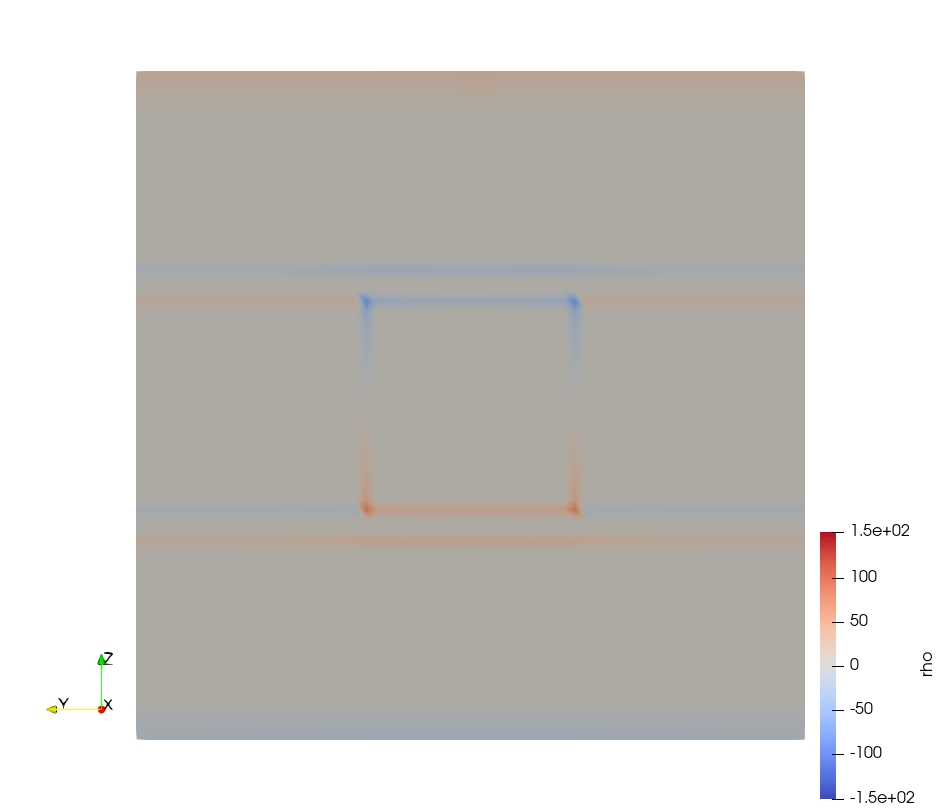
\includegraphics[scale=0.2]{Images/4.rho_3d.jpeg}
   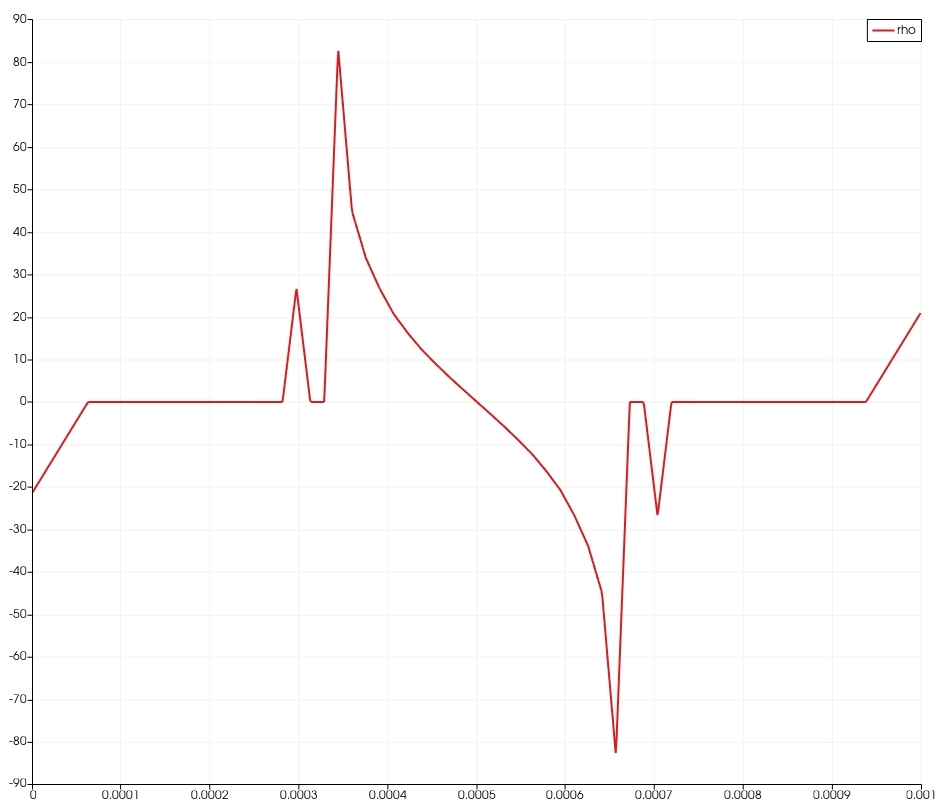
\includegraphics[scale=0.2]{Images/4.rho_new.jpeg}
    \caption {Test 4: charge density in the cube (left) and as a function of the z coordinate (right) for a line that intersects the left face of the cavity and at $t=T$.}
    \label{fig: 4.2}
\end{figure}
The charge density around the butt-gap is not uniform: if Figure \ref{fig: 4.2.1} we show the values of $\rho$ plotted over a line parallel to the x-axes, the first one passing through the bottom-left edge, the second one across the bottom face.
\begin{figure}[h!]
    \centering
   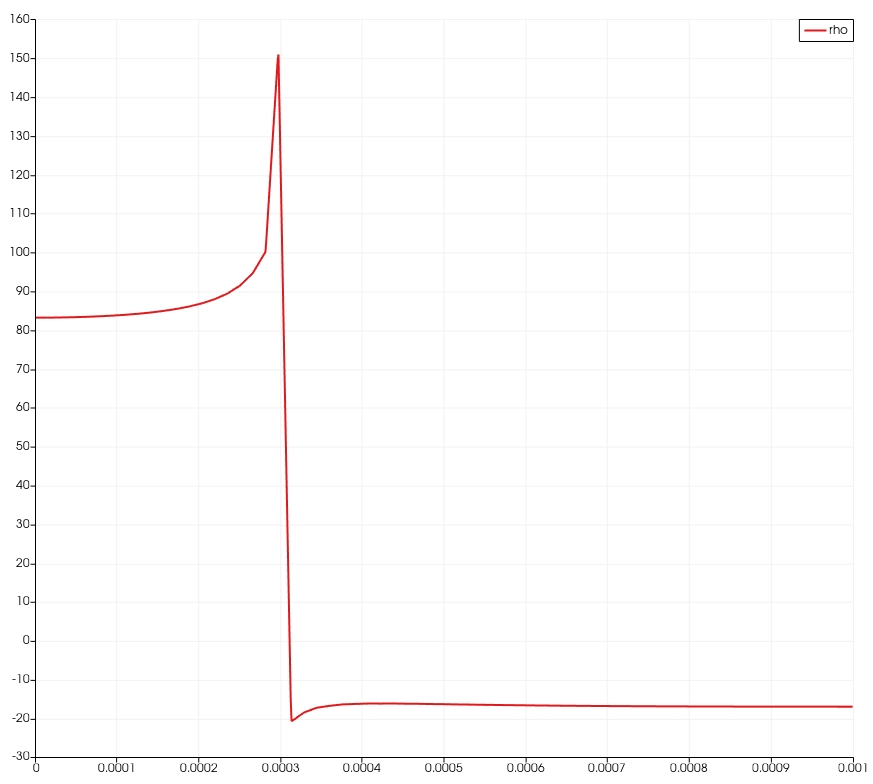
\includegraphics[scale=0.2]{Images/4.rho_x.jpeg}
   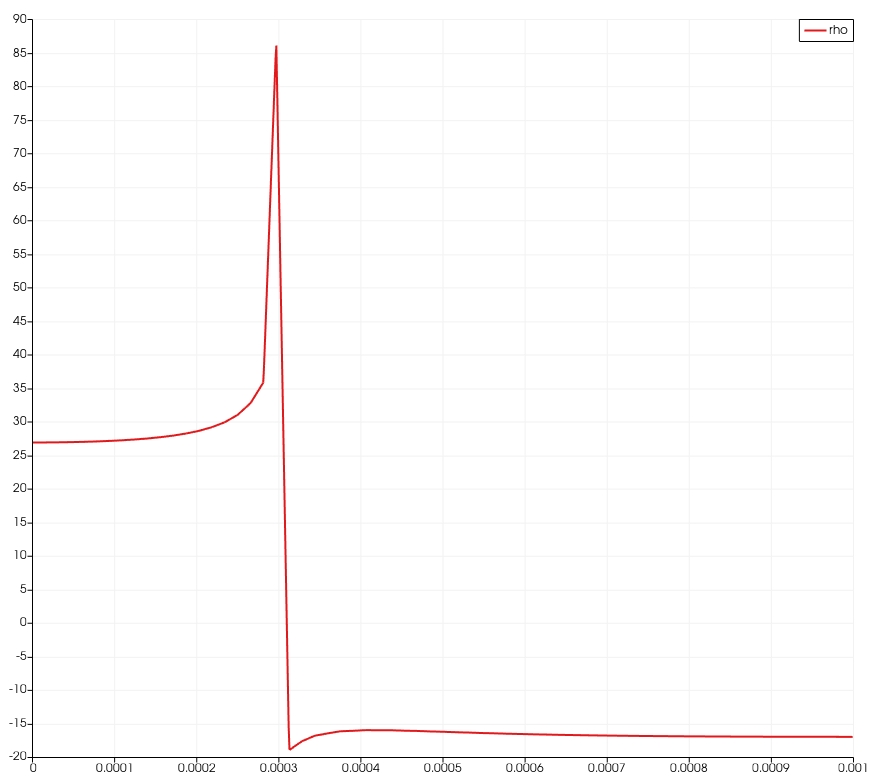
\includegraphics[scale=0.2]{Images/4.rho_x2.jpeg}
    \caption {Test 4: charge density in the cube plotted over lines parallel to the x-axis at $t=T$.}
    \label{fig: 4.2.1}
\end{figure}
\\In Figure \ref{fig: 4.2.2} we represent the $\rho$ plotted over a line parallel to the y-axes, the first one passing through the front-bottom edge, the second one across the bottom face.
\begin{figure}[h!]
    \centering
   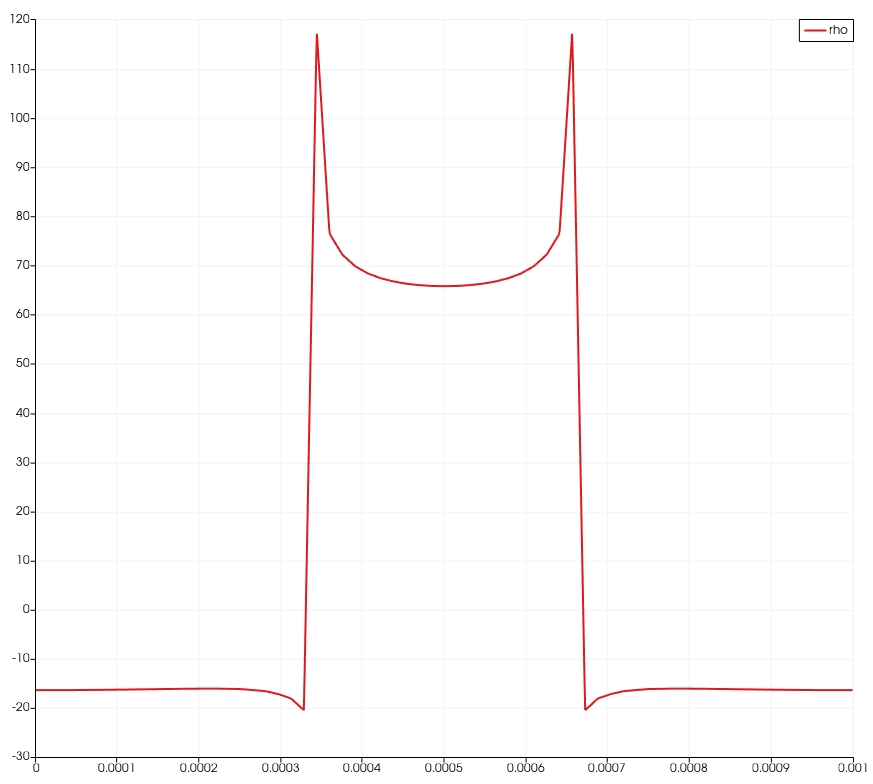
\includegraphics[scale=0.2]{Images/4.rho_y2.jpeg}
   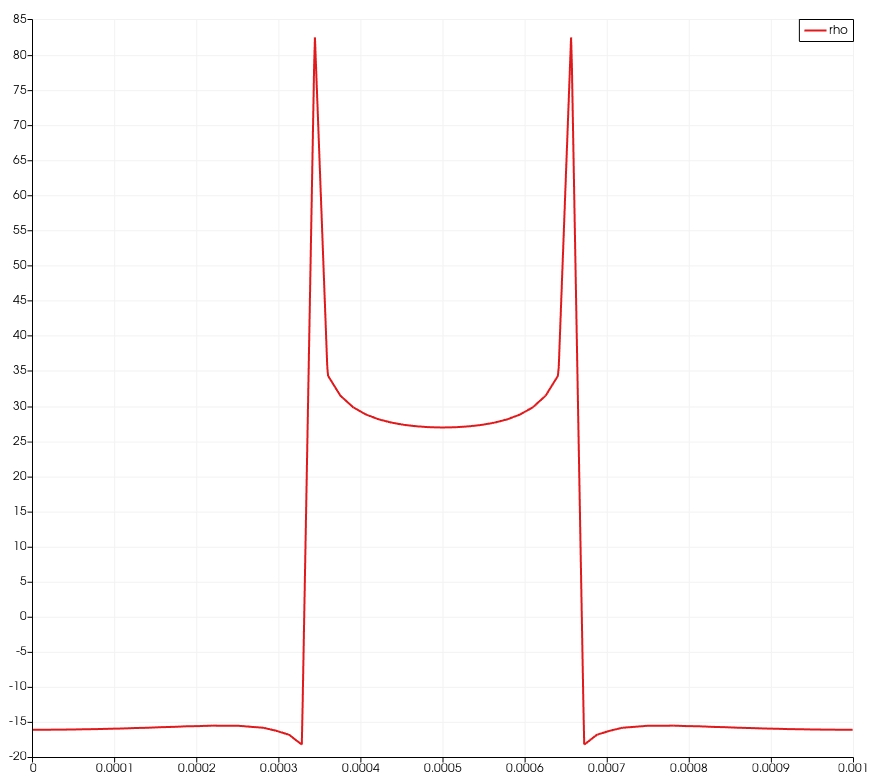
\includegraphics[scale=0.2]{Images/4.rho_y.jpeg}
    \caption {Test 4: charge density in the cube plotted over lines parallel to the y-axis at $t=T$.}
    \label{fig: 4.2.2}
\end{figure}
From the previous plots we can see that we have a high charge accumulation at the vertices of the cavity and also at the air-oil interfaces.
\\In Figure \ref{fig: 4.3} we represent the charge values at different points over time. We can see that the charge accumulate at different rates, with the top face ($\sigma_1$) being the fastest and the first paper-oil interface ($\sigma_2$) the slowest. Moreover, we can see that the highest $\rho$ value is achieved at the back-bottom edge ($\sigma_6$), where oil, air and paper are present.
\begin{figure}[h!]
    \centering
   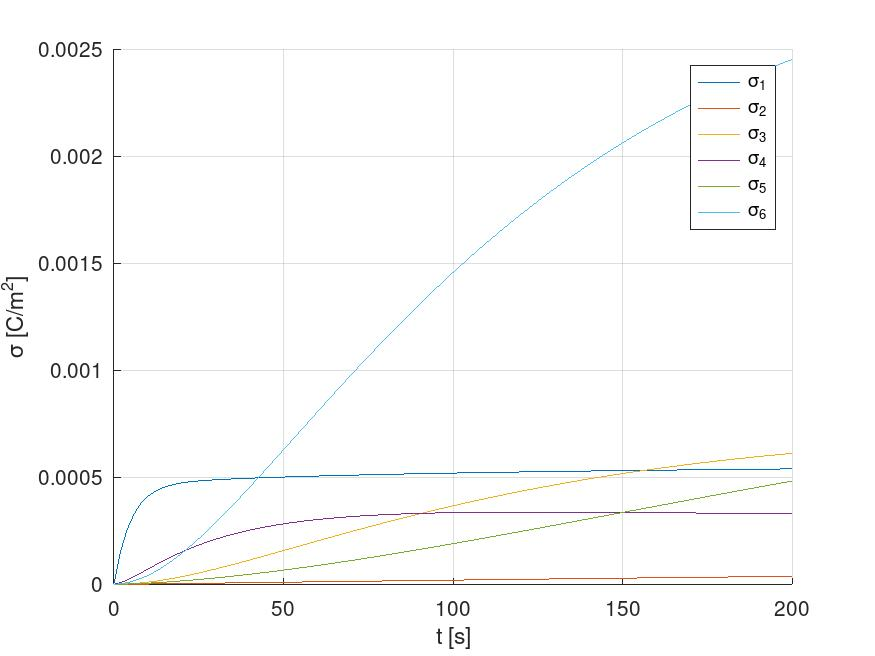
\includegraphics[scale=0.2]{Images/4.rho_time_fast_new.jpeg}
   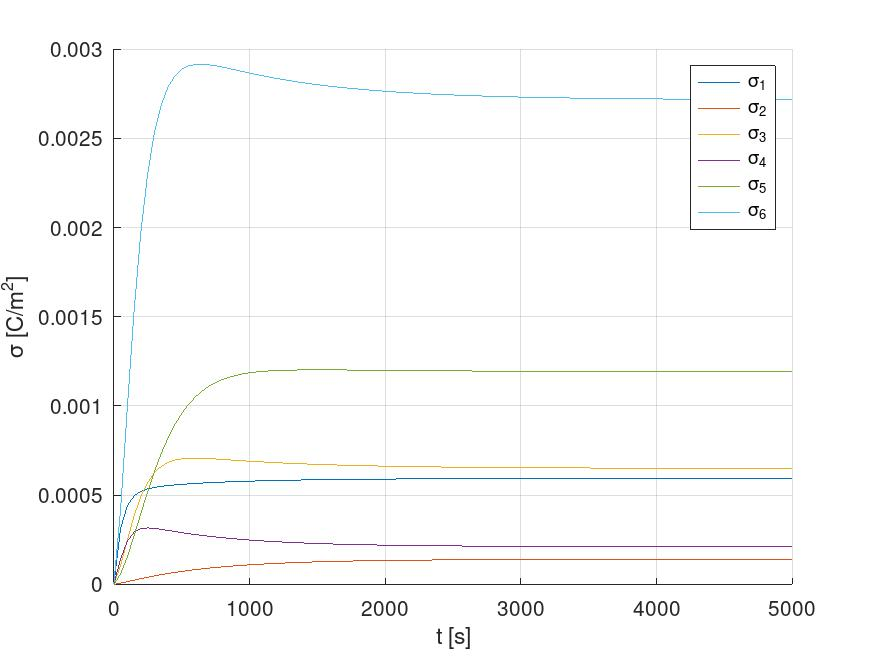
\includegraphics[scale=0.2]{Images/4.rho_time_new.jpeg}
    \caption {Test 4: charge density as a function of time: the left plot is computed with parameters $T=200,\ \Delta t=2,\ \tau=5$, the right one with $T=5000,\ \Delta t=50,\ \tau=50$. $\sigma_1$ represents the upper interface, $\sigma_2$ the first paper-oil interface, $\sigma_3$ the front-bottom-left vertex of the cavity, $\sigma_4$ the centre of the lower face, $\sigma_5$ the back-bottom-left vertex and $\sigma_6$ represents the centre of the back-bottom edge of the butt-gap.}
    \label{fig: 4.3}
\end{figure}

\section{Test 5}
In Test 3 we to simulate the behaviour of o polymeric insulator with a spherical air-filled cavity inside, which represents the damage of the material due to the conduction current. We consider a cubic domain with homogeneous permittivity, but for a semi-spherical cavity filled with air, with parameters $\epsilon_r=1$ and $\sigma=1e-12$.
The mesh has refinement of level $N_\text{ref}=4$, and $N_\text{ref,loc}=8$ around the sphere. (Figure \ref{fig: 5.1}).
\begin{figure}[h!]
    \centering
   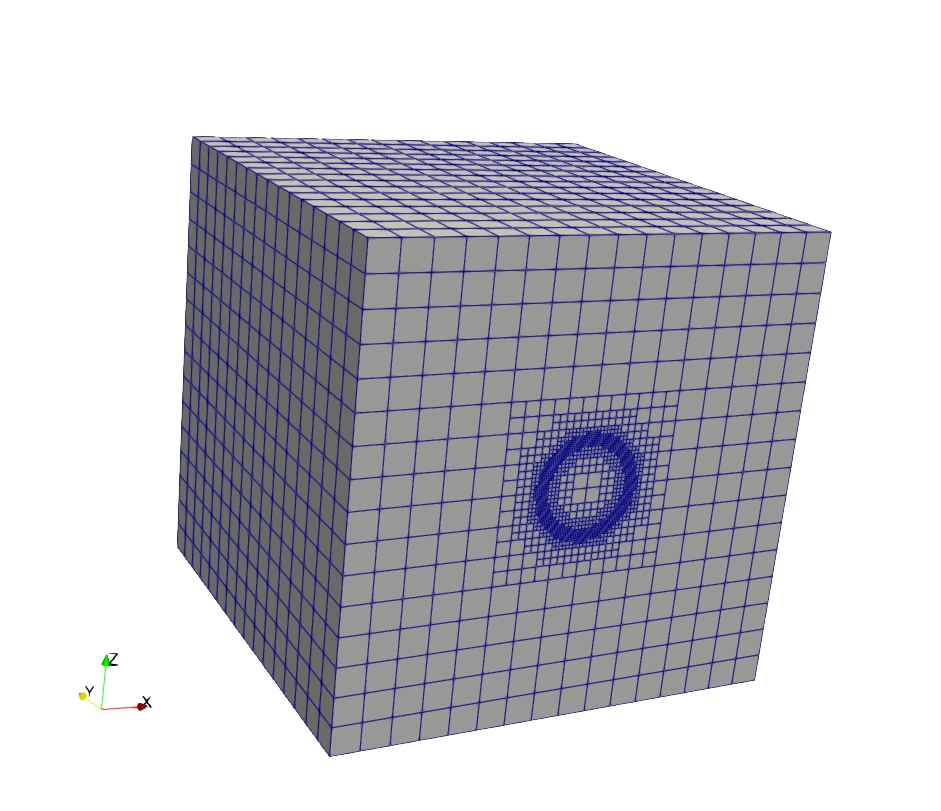
\includegraphics[scale=0.25]{Images/5.grid.jpeg}
    \caption {Test 5: mesh with local refinement of level $N_\text{ref}=8$ around the sphere, $N_\text{ref}=4$ elsewhere.}
    \label{fig: 5.1}
\end{figure}
\\The electric field is shown in Figure \ref{fig: 5.2}: we can see a sharp change of the gradient corresponding to the position of the sphere. 
\begin{figure}[h!]
    \centering
   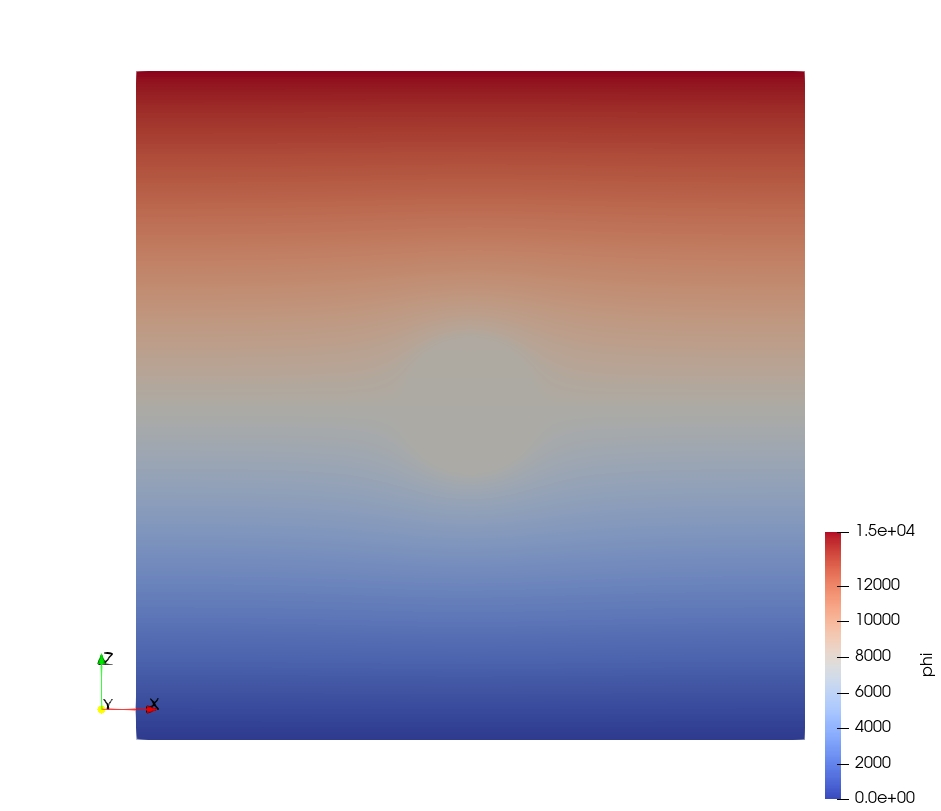
\includegraphics[scale=0.2]{Images/5.phi_3d.jpeg}
   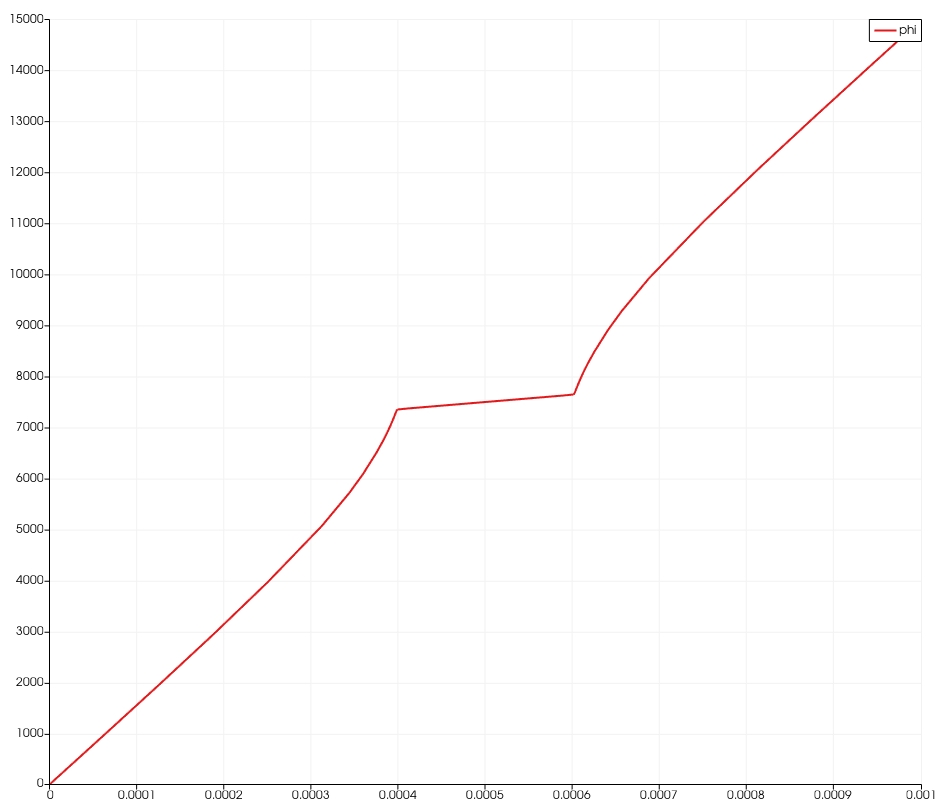
\includegraphics[scale=0.2]{Images/5.phi.jpeg}
    \caption {Test 5: electric potential in the cube (left) and as a function of the z coordinate (right) for $t=T$.}
    \label{fig: 5.2}
\end{figure}
\\In Figure \ref{fig: 5.3} we can see that we have an accumulation of charge on the border of the sphere. In particular, the charge density is greater in magnitude near the top and bottom of the sphere, and goes to 0 on the sides.
\begin{figure}[h!]
    \centering
   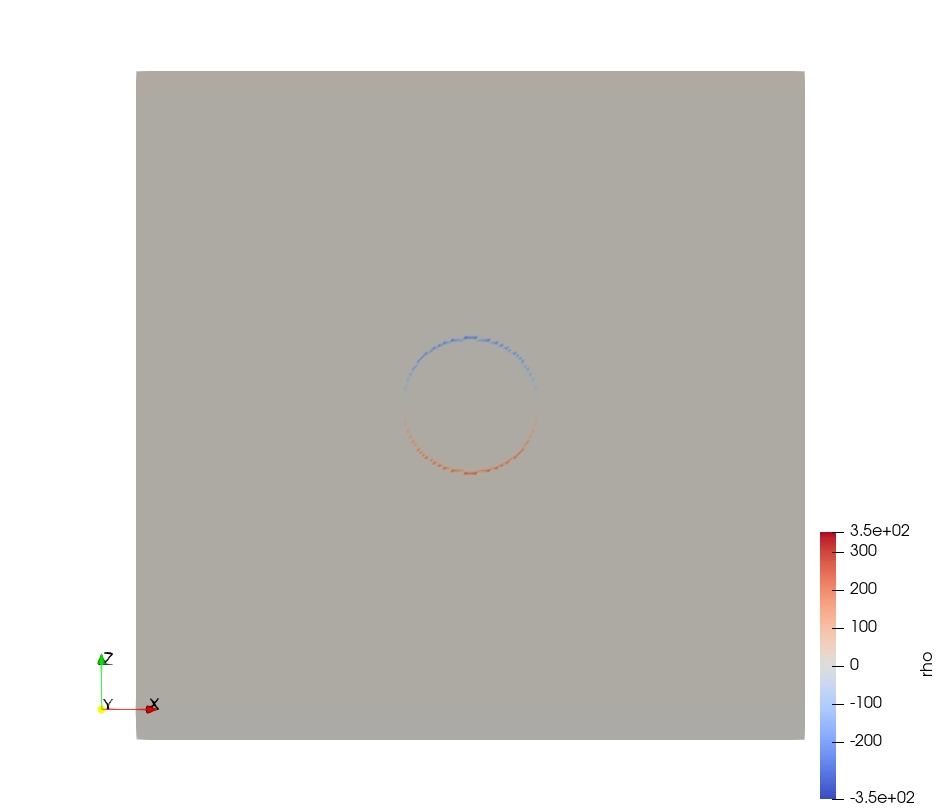
\includegraphics[scale=0.2]{Images/5.rho_3d.jpeg}
   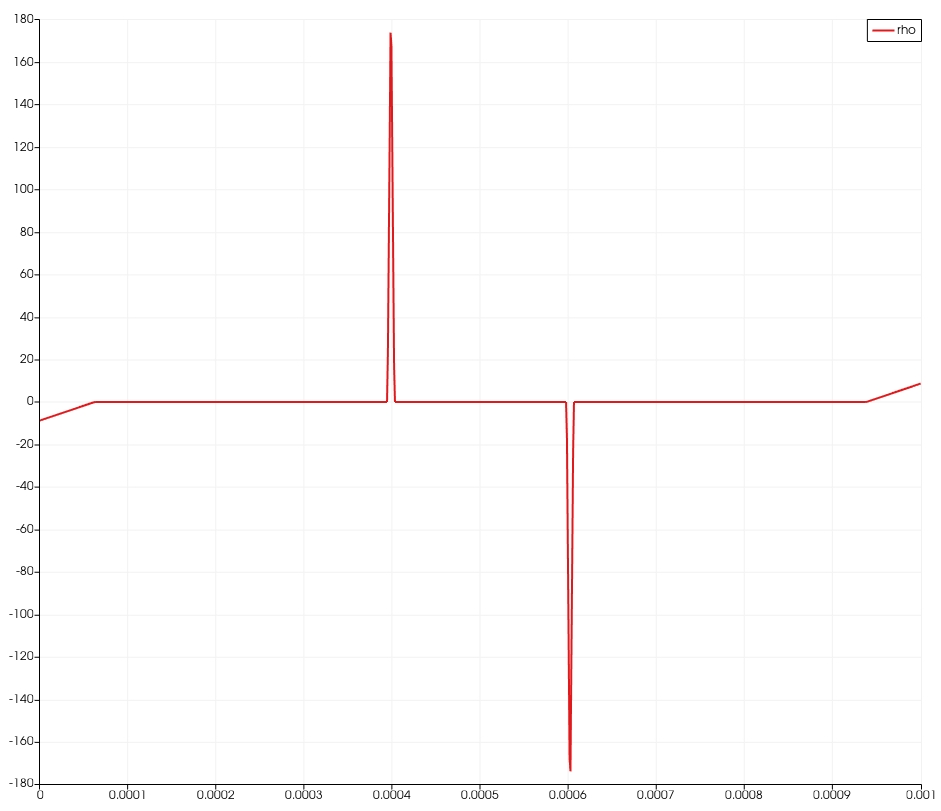
\includegraphics[scale=0.2]{Images/5.rho.jpeg}
    \caption {Test 5: charge density in the cube (left) and as a function of the z coordinate (right) for $t=T$.}
    \label{fig: 5.3}
\end{figure}
\\In Figure \ref{fig: 5.4} we show that the charge accumulates more slowly on the sphere compared to the upper and lower interfaces of the domain.
\begin{figure}[h!]
    \centering
   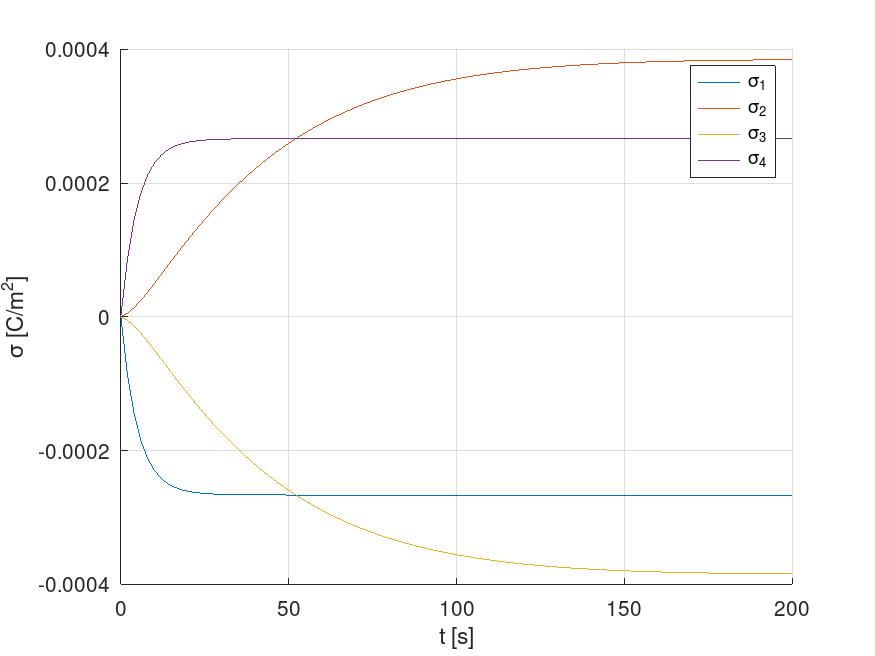
\includegraphics[scale=0.2]{Images/5.rho_time.jpeg}
    \caption {Test 5: charge density as a function of time: the plot is computed with parameters $T=200,\ \Delta t=2,\ \tau=5$. $\sigma_1$ represents the lower interface, $\sigma_2$ the bottom and $\sigma_3$ the bottom and top of the sphere, $\sigma_4$ represents the upper interface.}
    \label{fig: 5.4}
\end{figure}

\chapter{Conclusions and future developments} 
In this project we implemented a solver for a system of PDEs which models the charge and electric potential inside a dielectric material. The obtained results are consistent with the theoretical ones, showing the validity of the mathematical model and of the implementation. We have shown how the presence of air inside the material leads to a greater accumulation of charge locally compared to other interfaces such as paper-oil or two dielectric materials.
The use of the bim++ library allows to speed up the computational time thanks to the parallelization, however more test on the scalability of the code are required.
\\The next step for this project would be to implement the higher complexity models Level 1 and Level 2, which are more computationally expensive but should yield result of higher accuracy when applied to polymeric insulators. Moreover, the analysis of the displacement and conduction currents could give a better understanding of the processes that lead to premature degradation of the materials involved.

%-------------------------------------------------------------------------
%	BIBLIOGRAPHY
%-------------------------------------------------------------------------

\addtocontents{toc}{\vspace{2em}} % Add a gap in the Contents, for aesthetics
\bibliography{Thesis_bibliography} % The references information are stored in the file named "Thesis_bibliography.bib"

\end{document}
